%!TEX root = ../dissertation.tex

\chapter{NONPARAMETRIC COVARIANCE FUNCTION AND PRINCIPAL COMPONENT FUNCTION ESTIMATION FOR FUNCTIONAL DATA}
\label{ch:covariance estimation}

\section{Abstract}
Functional principal components are often used in exploratory analysis and as a modeling tool. As in multivariate methods, functional principal components are derived from the covariance function. By using a reproducing kernel Hilbert space framework, it has been shown that efficient covariance function estimation is achieved through a regularization approach on the tensor product space. We adopt this framework and show how this method can be extended to allow for unpenalized subspaces which arise naturally when the smoothing penalty is based on a high order derivatives.  Closed form estimators of the principal component functions are also derived without discretizing the covariance function, making this method ideally suited for use as an empirical basis set for functional data analysis.

\section{Introduction}
Functional principal components are often used in exploratory analysis and as a modeling tool. In multivariate methods, principal components are derived through an eigen-decomposition of the covariance; however, with functional data the covariance is not a matrix, but a continuous bivariate function. \cite{Cai:2010vr} propose a framework for nonparametric covariance function estimation for a second order stochastic process, $X(\cdot)$, with support on a compact domain $\T\subset \Real$ and $X(\cdot) \in \H$, where $\H$ is a reproducing kernel Hilbert space. By examining the form of the covariance function within this framework, it can be shown that the covariance function resides in the tensor product reproducing kernel Hilbert space $\H\otimes \H$. Based on this fact, it is natural to consider a regularization procedure for covariance function estimation that utilizes the tensor product norm. \cite{Cai:2010vr} proposed the following
\begin{equation}
\hat{C}_{\lambda}=\stackrel[C \in \H\otimes\H]{}{\mbox{argmin}} \{l_{n}(C)+\lambda\left\Vert C\right\Vert _{\H\otimes \H}^{2}\},
\end{equation}
 where
\begin{equation}
l_{n}(C)=\sum_{i=1}^{n}\sum_{1\leq j_{1}\neq j_{2}\leq m}([Y_{ij_{1}}-\mu_{0}(t_{ij})][Y_{ij_{2}}-\mu_{0}(t_{ij_{2}})]-C(t_{ij_{1}},t_{ij_{2}}))^{2}
\label{eq:loss}
\end{equation}
 and $\lambda\geq0$ is a tuning parameter that balances the fidelity
to the data measured by $l_{n}$ and smoothness of the estimate measured
by the squared RKHS norm.

The convergence rate of this estimator has been shown to be superior to the optimal rate for general bivariate smoothing on $[0,1]\times[0,1]$. This implies that the tensor product RKHS is to a certain degree smaller than the typical Sobelev space used for bivariate smoothing, thus reducing the effect of ``the curse of dimensionality''. 

By establishing a representer theorem (see \cite{Wahba:1990}), the covariance function estimator has a finite dimensional representation. Further, using this representation, closed form expressions for the eigenfunctions can be derived. These developments provide a strong argument for the use of reproducing kernel Hilbert space framework when interest is in nonparametric estimation of the covariance function and principal component functions. 

This approach assumes that the reproducing kernel is known and that the tensor product norm corresponding to the reproducing kernel penalizes smoothness in an appropriate way. It seems important, from a practical point of view, to have a clear understanding of how the penalty functional is operating. To accomplish this we propose an approach that begins with defining how univariate functions are penalized on the marginal domain (typically done by defining an appropriate high order derivative), then use the implied penalty on the tensor product domain to estimate the covariance function. This approach is more attractive from a practitioner's point of view, because it is more natural to define a differential operator to penalize smoothness, and in this case the functions annihilated by the differential operator form a non-null subspace. Our approach allows for a decomposition of the function space into penalized and unpenalized subspaces. To illustrate this, recall the general development for the smoothing spline in the univariate case (\cite{Wahba:1990}):  The solution of 
\begin{equation}
\widehat{f}_{\lambda} = \hspace{.07in}\stackrel[f \in \H]{}{\mbox{argmin}} \left\{ \frac{1}{n}\sum_{i=1}^{n}(y_i - f(t_i))^2 + \lambda\norm{f}^2_{\H} \right\}
\end{equation}
has the form
\begin{equation}
	\hat{f}(t) = \sum_{i=1}^N c_iR(t, t_i), 
\end{equation}
while the solution of
\begin{equation}
\widehat{f}_{\lambda} = \hspace{.07in}\stackrel[f \in \H]{}{\mbox{argmin}} \left\{ \frac{1}{n}\sum_{i=1}^{n}(y_i - f(t_i))^2 + \lambda\norm{P_1(f)}^2_{\H_1} \right\}
\label{eq:unpenalized objective function}
\end{equation}
has the form
\begin{equation}
	\hat{f}(t) = \sum_{j=1}^M d_j\phi_j(t) + \sum_{i=1}^N c_iR_1(t, t_i), 
	\label{eq:unpenalized solution}
\end{equation}
where $\{\phi_j(\cdot)\}_{j=1}^M$ are a basis for the space of unpenalized functions $\H_0$ and $P_1(f)=f_1$ is the projection of $f$ onto the space $\H_1$. For details of the derivation of \eqref{eq:unpenalized solution} from \eqref{eq:unpenalized objective function} see section~\ref{sec:theoretical background}. 
In Section \ref{covariance estimation} we generalize regularization procedure for covariance function in \cite{Cai:2010vr} to account for this type of decomposition.  In Section \ref{eigenfunctions} we derive closed form estimators of the principal component functions based on the generalized covariance estimator.

\section{Methodology}

 In the following we assume $\T$ to be the interval $[0,1]$. Let $X(\cdot)$ be a second order stochastic process with covariance function
 \[
C_{0}(s,t)=E([X(s)-E(X(s))][X(t)-E(X(t))]),\mbox{  }\forall s,t\in \T.
\]
Further, assume $X(\cdot)$ takes values in a reproducing kernel Hilbert space (RKHS) $\H$ with corresponding reproducing kernel $R(s,t)$. The reproducing kernel $R(s,t)$ has the property $\inner{f(s)}{R_t(s)}_{\H} = f(t)$ for all $f \in \H$, where $R_t(s)$ is notation for $R(s,t)$ holding the second coordinate fixed. The function $R_t(s)$  belongs to $\H$; as an immediate consequence of the reproducing property $\inner{R_{t_1}(s)}{R_{t_2}(s)} = R(t_1, t_2)$. This is a key property, since it shows that inner products involving the reproducing kernel function are equivalent to function evaluation.  

Let $\{X_{1},X_{2},\dots,X_{N}\}$ be a collection of independent realizations
of $X$, and we consider the following observation model
\[
Y_{ij}=X_{i}(t_{ij})+\epsilon_{ij},\mbox{   }j=1,\dots,m;\mbox{ }i=1,\dots,N,
\]
where the sampling locations are independently drawn from a common
distribution on $\T,$ and $\epsilon_{ij}$ are independently and identically
distributed measurement errors with mean zero and finite variance
$\sigma_{0}^{2}.$ It is further assumed that the random functions
$X,$ sampling locations $t_{ij},$ and measurement errors $\epsilon$ are
mutually independent. 

The development in this section relies on the fact that a closed subspace of a Hilbert space induces a natural partition of the space into a direct sum of the closed subspace and its orthogonal complement (for a concise overview of the relevant Hilbert space theory, see \cite{Gu2002}). The subspace consisting unpenalized functions is a closed subspace and it is convenient to express $\H$ as a direct sum decomposition $\H = \H_0 \oplus \H_1$, where on $\H_1$ the penalty functional is a full squared norm and $\H_0$ consists of functions in $\H$ which will not be penalized. With this orthogonal decomposition, any function $f \in \H$ has the representation $f = f_0 + f_1$, where $f_0 \in \H_0$ and $f_1 \in \H_1$. 
 A well known result (see Theorem \ref{RKHS_decomposition}), is that the reproducing kernel $R$ on $\H$ can be expressed as $R = R_0 + R_1$, where $R_0$ is the reproducing kernel on $\H_0$ and $R_1$ is the reproducing kernel on $\H_1$.


Covariance function estimation takes place on the product domain $[0,1]\times[0,1]$ = $\T_1\times \T_2$. Denote by $\H_{<1>}$ and $\H_{<2>}$  the reproducing kernel Hilbert space on $\T_1$ and $\T_2$, respectively.  Let $\H_{<1>}=\H_{0<1>} \oplus\H_{1<1>}$ and $\H_{<2>} = \H_{0<2>} \oplus \H_{1<2>}$ be the direct sum decomposition of spaces on the marginal domains into their unpenalized and penalized subspaces. Using these decompositions, the tensor product space $\H_{<1>} \otimes \H_{<2>}$ has the representation
\begin{align}
	\H_{<1>} \otimes \H_{<2>} &=( \H_{0<1>} \oplus \H_{1<1>}) \otimes (\H_{0<2>} \oplus \H_{1<2>})\\
						 &= ( \H_{0<1>}  \otimes\H_{0<2>}) \oplus (\H_{0<1>}   \otimes \H_{1<2>}) \oplus ( \H_{1<1>}  \otimes \H_{0<2>})   \oplus (\H_{1<1>}  \otimes  \H_{1<2>}) \label{eq:tpsum}
\end{align}

Equation \eqref{eq:tpsum} is a direct sum of tensor product reproducing kernel Hilbert spaces, where the subspace corresponding to $ \H_{0<1>}  \otimes\H_{0<2>}$ consists only of unpenalized functions. As in the univariate case, the solution to the penalized smoothing problem when unpenalized subspaces are allowed will involve linear combination of the basis functions for the unpenalized subspace. 

The main goal in what follows is to describe the form of the covariance function estimator when the tensor product space has a decomposition as in \eqref{eq:tpsum}. This setting is more attractive from a practitioner's point of view, because it is more natural to define a differential operator to penalize smoothness, and in this case the functions annihilated by the differential operator form a non-null subspace. We describe the form of the estimator in this case as well as derive the principle component functions. Since our focus is on practical implementation of this method, we focus on the most common case where the smoothing penalty on the marginal domain is $\int(f'')^2$, i.e. the total curvature.

 %====================================================
 \section{Covariance function estimation} \label{covariance estimation}
  %====================================================
  
Consider the space $\H =  \{f : f, f' \mbox{ absolutely continuous}, f'' \in L_2[0,1]\}$. On this space the term $\int_0^1 f''g''dx$ is a semi-inner-product which can be extended to a full inner product by defining an inner product on the subspace $\H_0 = \{f : f'' = 0\}$. Common choices for inner products in $\H_0$ are $\inner{f}{g}_0 = f(0)g(0) + f'(0)g'(0)$ or $\inner{f}{g}_0 = (\int_0^1fdx)(\int_0^1gdx) + (\int_0^1f'dx)(\int_0^1g'dx)$. We work with the latter because it corresponds to a mathematically convenient expression for the reproducing kernel. 
  
  The space $\H =  \{f : f, f' \mbox{ absolutely continuous}, f'' \in L_2[0,1]\}$ with inner product
  \begin{align*}
  \inner{f}{g} &= \inner{f}{g}_0 + \inner{f}{g}_1 \\
  			&= \left(\int_0^1fdx\right)\left(\int_0^1gdx\right) + \left(\int_0^1f'dx\right)\left(\int_0^1g'dx\right) + \int_0^1 f''g''dx
  \end{align*}�
  is a RKHS with a reproducing kernel that can be conveniently expressed in terms of the functions
  \begin{equation}
  k_r(x) = -\left( \sum_{\mu = -\infty}^{-1} + \sum_{\mu=1}^{\infty} \right) \frac{\exp(2\pi i \mu x)}{(2 \pi i \mu)^r}, r = 1,2, \dots.
  \label{eq:kfuns}
  \end{equation}�
  The functions $k_r(x)$ in \eqref{eq:kfuns} are scaled Bernoulli polynomials, $k_r(x) = \frac{B(r)}{r!}$. The space $\H$ has an orthogonal decomposition $\H = \H_0 \tsum \H_1$ with corresponding reproducing kernel $R(x,y) = R_0(x,y) + R_1(x,y)$, where
  \begin{align}
  R_0(x,y) &= 1 + k_1(x)k_1(y) \\
  R_1(x,y) &= k_2(x)k_2(y) - k_4(x-y).
  \end{align}�
  Note that the functions  $k_r(x)$ in \eqref{eq:kfuns}  have a rather simple form
  \begin{align*}
  k_1(x) &= x - 0.5\\
  k_2(x) &= \frac{1}{2}(k_1^2(x) - \frac{1}{12}) \\
  k_4(x) &= \frac{1}{24} \left(k_1^4(x) - \frac{k_1^2(x)}{2} + \frac{7}{240} \right)
  \end{align*}�
  for $x \in [0,1]$. 
  
  The unpenalized space $\H_0$ can be decomposed further as $\H_0 = \H_{00} \tsum \H_{01}$ with reproducing kernels
  \begin{align*}
  �R_{00}(x,y) &= 1\\
   R_{01}(x,y) &= k_1(x)k_1(y).\\
  \end{align*}� 
This formulation provides a decomposition of the unpenalized space into functions spanned by a constant and functions spanned by a linear term. This construction results in the overall decomposition $\H= \H_{00} \tsum \H_{01} \tsum \H_1$. Using this decomposition of $\H$ on both marginal domains of $[0,1] \times [0,1]$ results in a natural decomposition of the tensor product space 
\[
\H_{<1>} \tprod \H_{<2>} = (\H_{00<1>} \tsum \H_{01<1>} \tsum \H_{1<1>})\tprod (\H_{00<2>} \tsum \H_{01<2>} \tsum \H_{1<2>})
\]
into a sum of nine subspaces of the tensor product space. These nine subspaces and their corresponding reproducing kernels are shown in Table \ref{tab:tp decomp}. It is straight forward to derive the reproducing kernels in Table \ref{tab:tp decamp} using the fact that the reproducing kernel on the tensor product space is the product of the reproducing kernels on the marginal spaces, i.e. $R((x_{<1>}, x_{<2>}), (y_{<1>}, y_{<2>}) ) = R_{<1>}(x_{<1>}, y_{<1>})\times R_{<2>}(x_{<2>}, y_{<2>})$.

\begin{table}[h]
\caption{Tensor product space decomposition with corresponding reproducing kernels.}
\label{tab:tp decomp}
\begin{tabular}{|c|c|}
\hline 
Subspace & Reproducing Kernel\tabularnewline
\hline
\hline 
$H_{00<1>}\otimes H_{00<2>}$ & 1\tabularnewline
\hline 
$H_{00<1>}\otimes H_{01<2>}$ & $k_{1}(x_{<2>})k_{1}(y_{<2>})$\tabularnewline
\hline 
$H_{00<1>}\otimes H_{1<2>}$ & $k_2(x_{<2>})k_2(y_{<2>}) - k_4(x_{<2>} - y_{<2>})$\tabularnewline
\hline 
$H_{01<1>}\otimes H_{00<2>}$ & $k_1(x_{<1>})k_1(y_{<1>})$ \tabularnewline
\hline 
$H_{01<1>}\otimes H_{01<2>}$ & $k_1(x_{<1>})k_1(y_{<1>})k_1(x_{<2>})k_1(y_{<2>})$ \tabularnewline
\hline 
$H_{01<1>}\otimes H_{1<2>}$ & $k_1(x_{<1>})k_1(y_{<1>})[k_2(x_{<2>})k_2(y_{<2>}) - k_4(x_{<2>} - y_{<2>})]$\tabularnewline
\hline 
$H_{1<1>}\otimes H_{00<2>}$ & $k_2(x_{<1>})k_2(y_{<1>}) - k_4(x_{<1>} - y_{<1>})$\tabularnewline
\hline 
$H_{1<1>}\otimes H_{01<2>}$ & $[k_2(x_{<1>})k_2(y_{<1>}) - k_4(x_{<1>} - y_{<1>})]k_1(x_{<1>})k_1(y_{<1>})$\tabularnewline
\hline 
$H_{1<1>}\otimes H_{1<2>}$ & $[k_2(x_{<1>})k_2(y_{<1>}) - k_4(x_{<1>} - y_{<1>})][k_2(x_{<2>})k_2(y_{<2>}) - k_4(x_{<2>} - y_{<2>})]$\tabularnewline
\hline
\end{tabular}
\end{table}

Of the tensor product subspaces listed in Table \ref{tab:tp decomp}, only five have $\H_1$ as one of their marginal domain spaces. If we denote $\H_{\nu, \mu}=\H_{\nu <1>}\otimes \H_{\mu <2>}$ and $R_{\nu, \mu}=R_{\nu <1>}R_{\mu <2>}$, then $\breve{R} = R_{1,00}+R_{1,01}+R_{00,1}+R_{01,1}+R_{1,1}$ is the reproducing kernel on $\breve{\H} =  \H_{1,00}\oplus\H_{1,01}\oplus\H_{00,1}\oplus\H_{01,1}\oplus\H_{1,1}$. The space $\breve{\H}$ contain all functions we wish to penalize.

Let $\mathbf{b}^{(i)} = [(y_{ij}-\mu(t_{ij}))(y_{ij'}-\mu(t_{ij'}))]_{1\leq j\neq j'\leq m}$, $i=1, \dots, n$. Let
\[
\mathbf{b} = (\mathbf{b}^{(1)T}, \mathbf{b}^{(2)T}, \dots, \mathbf{b}^{(n)T}   )^T,
\]
then the vectors $\mathbf{b}^{(i)}$ contain all pairwise products of observations on the $i$th curve. We propose the following estimator
\[
\widehat{C}_{\lambda}=\stackrel[C \in \H\otimes \H]{}{\text{ argmin}} \left\{ (\mathbf{b} - \mathbf{C})^T(\mathbf{b} - \mathbf{C})+\lambda\left\Vert C\right\Vert _{\breve{\H}}^{2} \right\},
\]
 where
%\begin{equation}
%l_{n}(C)= (\mathbf{b} - \mathbf{C})^T(\mathbf{b} - \mathbf{C})
%\label{eq:loss1}
%\end{equation}
%and 
\[
\mathbf{C} = [C(t_{i,j}, t_{i'j'})].
\]

 
Using the representer theorem in \cite{Wahba:1990} theorem 1.3.1, it can be shown that the estimated covariance function has the form
\begin{equation}
		\hat{C}(s,t) = \sum_{\nu, \mu=00,01}d_{\nu,\mu}\phi_{\nu,\mu}(s,t) + \sum_{i,j}c_{i,j}\breve{R}((t_i,t_j),(s,t))
%\label{eq:}
\end{equation}
 The four basis functions for the unpenalized space are $\phi_{\nu,\mu}$ are $\{ 1, k_1(s), k_1(t), k_1(s)k_1(t)  \}$, so the solution can be written more explicitly as 
\begin{equation}
		\hat{C}(s,t) = d_{00,00} + d_{01,00}k_1(t) + d_{00,01}k_1(s) + d_{01,01}k_1(s)k_1(t) + \sum_{i,j}c_{i,j}\breve{R}((t_i,t_j),(s,t)). 
\label{eq:covest}
\end{equation}
Efficient estimation of \eqref{eq:covest} including smoothing parameter selection can be accomplished using methods described in \cite{Gu2002}.
%\todo{include the quadratic form version of the minimization problem}

%The estimator in \eqref{eq:covest} involves slices of the reproducing kernel on the penalized space. These slices are 2-dimensional surfaces and it is of some interest to investigate these surfaces. Figure~\ref{fig:basis_fns} shows some of these functions corresponding to knot locations on a five by five grid. 


 In practice the number of observed pairs $(t_i, t_j)$ will be large and we may want to specify the knot locations instead of using the observed locations. \cite{CFZ} recommend using knot locations forming a regular grid within the convex hull of the observed points. Let $t_i \in [0,1]; i=1,\dots, K$ be the chosen knot locations on the univariate space, making  $(t_i,t_j)_{1\leq i,j \leq K}$ a regular grid of knot locations on $[0,1]\times[0,1]$. \cite{Kim:2004tt} investigate this with a simulation study and give a general recommendation of $10n^{2/9}$, where $n$ is the sample size on the tensor product domain. 


%These functions have overlapping support, which why you should not use the data as knots for large data sets. 

%\begin{figure}%
%\centering
%\subfigure{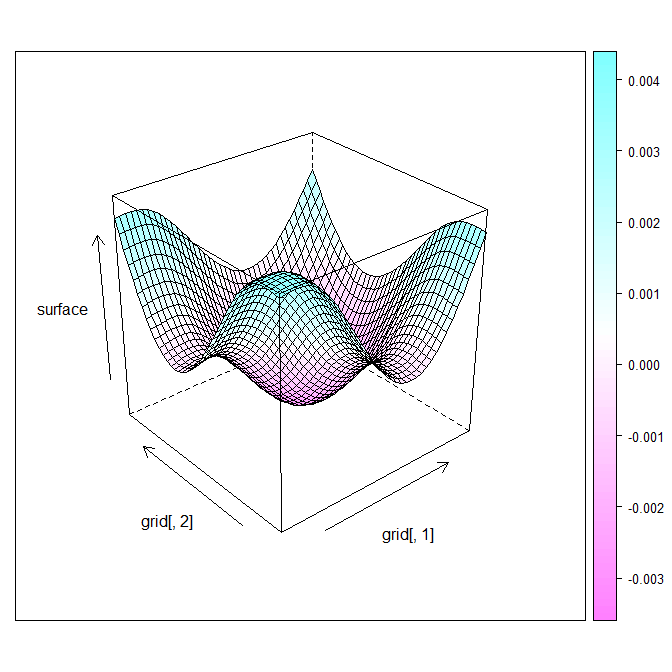
\includegraphics[width=.25\textwidth]{Images//basis_fn1.png}}
%\subfigure{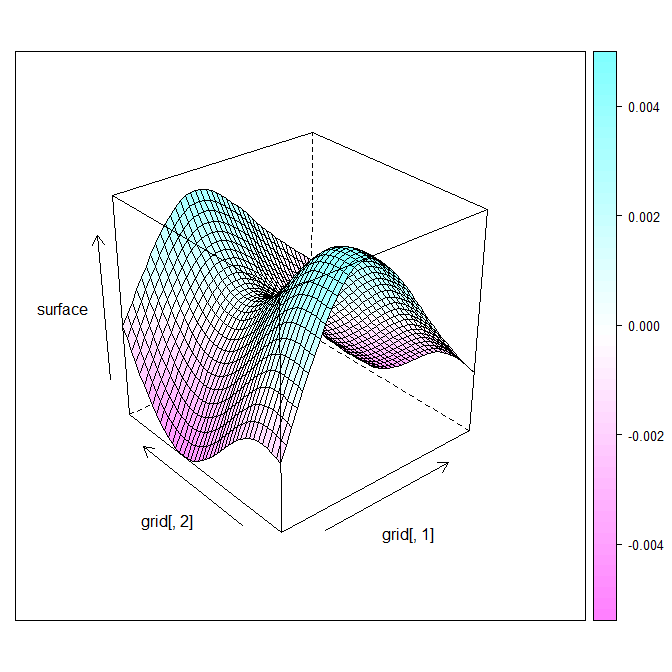
\includegraphics[width=.25\textwidth]{Images//basis_fn2.png}}
%\subfigure{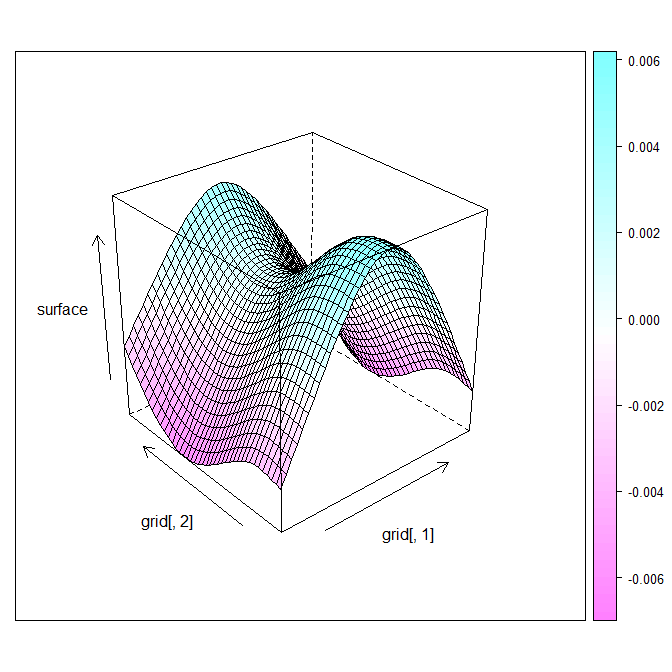
\includegraphics[width=.25\textwidth]{Images//basis_fn3.png}}
%\subfigure{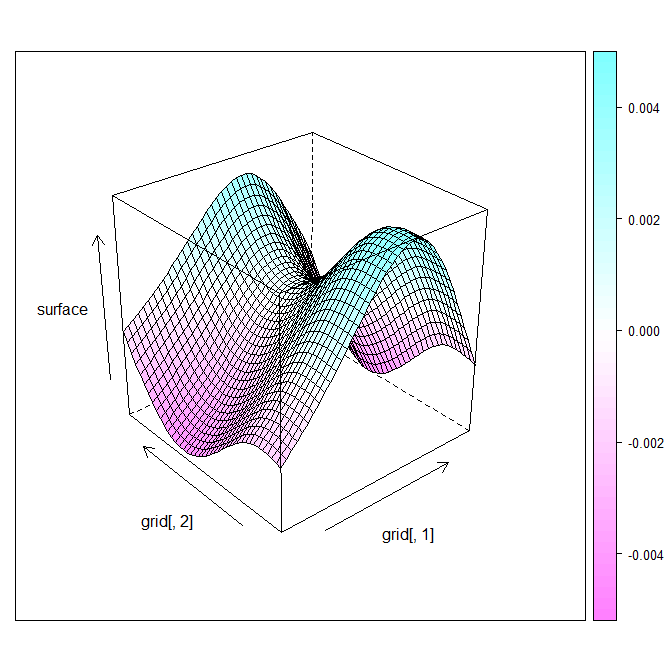
\includegraphics[width=.25\textwidth]{Images//basis_fn4.png}}
%\subfigure{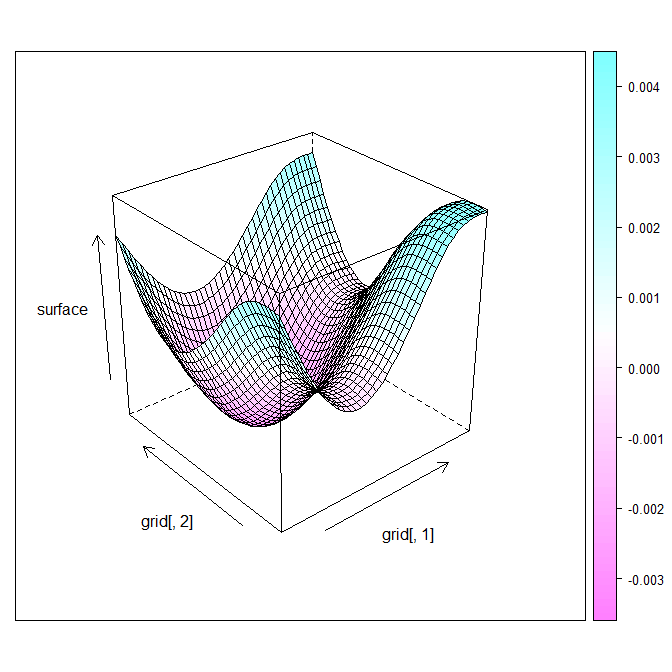
\includegraphics[width=.25\textwidth]{Images//basis_fn5.png}}
%\subfigure{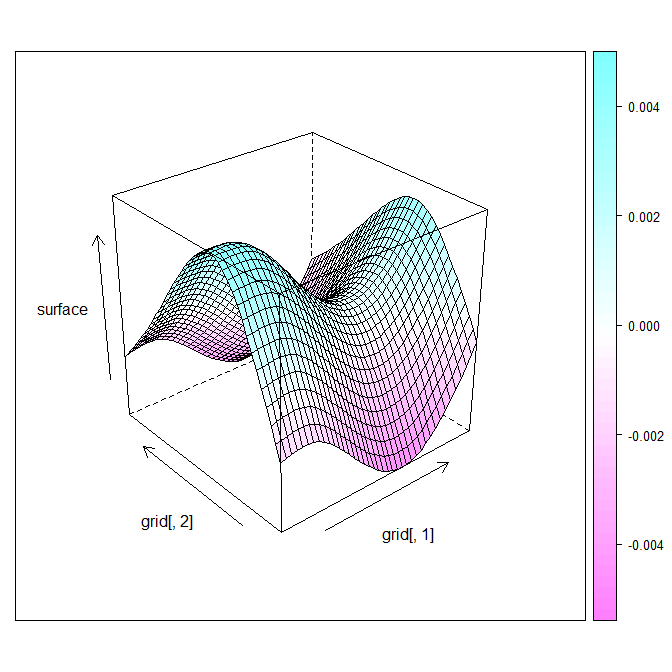
\includegraphics[width=.25\textwidth]{Images//basis_fn6.png}}
%\subfigure{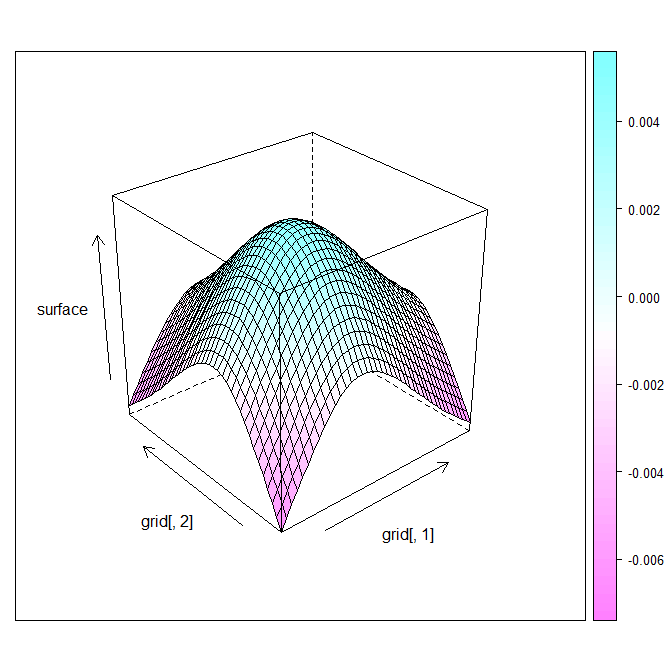
\includegraphics[width=.25\textwidth]{Images//basis_fn7.png}}
%\subfigure{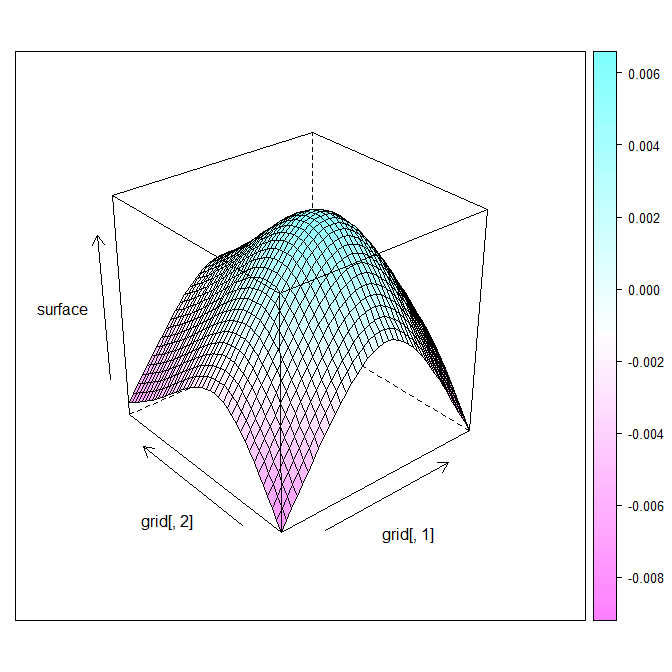
\includegraphics[width=.25\textwidth]{Images//basis_fn8.png}}
%\subfigure{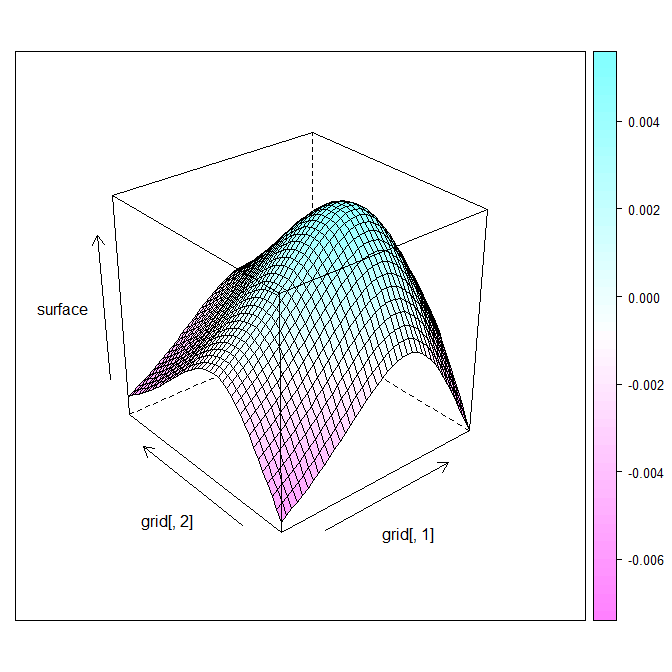
\includegraphics[width=.25\textwidth]{Images//basis_fn9.png}}
%\subfigure{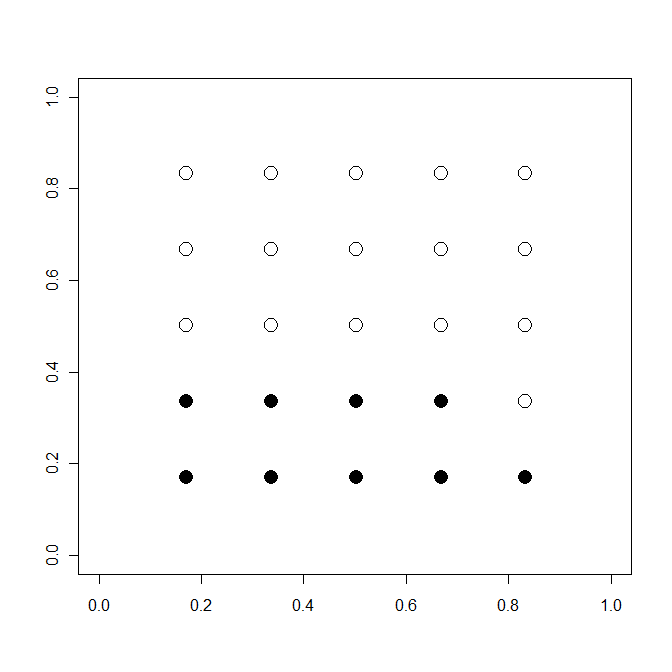
\includegraphics[width=.4\textwidth]{Images//knot_locations.png}}
%\caption{Plots of some of the basis functions in the penalized space. The plot on the bottom shows the corresponding knot location for each of the basis functions. The location of the black dot on the bottom left produced the basis function on the top left. The location of the black dot on the top right produced the basis function on the bottom right. }%
%\label{fig:basis_fns}%
%\end{figure}

%
%\begin{figure}%
%\centering
%\subfigure{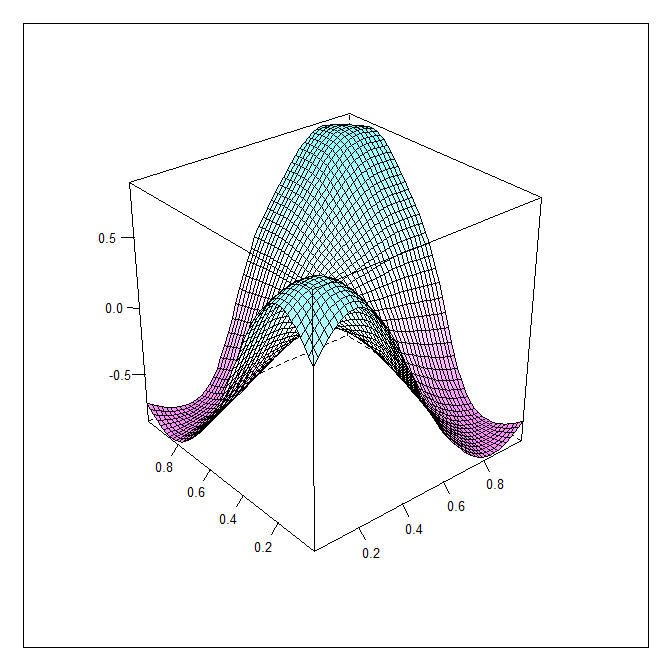
\includegraphics[width=.3\textwidth]{Images//est_cov.png}}
%\subfigure{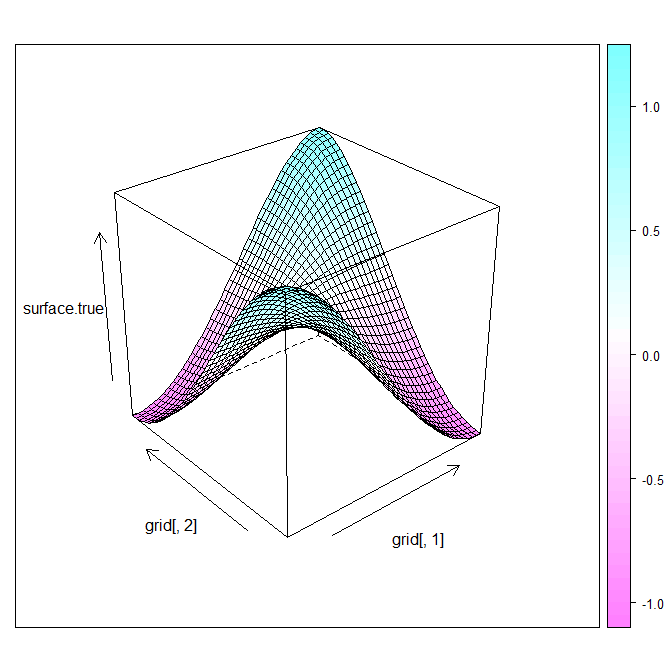
\includegraphics[width=.31\textwidth]{Images//true_cov.png}}
%\caption{Plot of estimated covariance function (left) and true covariance function (right). }%
%\label{fig:cov_est}%
%\end{figure}

%==========================================================
\section{Estimation of functional principal components } \label{eigenfunctions}
%==========================================================

Functional principal components are related to the well-known Karhunen-Loeve representation theorem. Here is a brief review of the relevant mathematical results.  

For a square-integrable stochastic process $X(t)$ defined on a closed interval $[a,b]$,  with continuous covariance $C(s,t)$, there corresponds a linear operator $[T_Cf](s) = \int_a^bC(s,t)f(t)dt$. Since $C(s,t)$ is symmetric and non-negative definite, it has the following representation (see Mercer's theorem)
\begin{equation*} 
 C(s,t) = \sum_{i=1}^{\infty}\lambda_i\psi_i(s)\psi_i(t),
\end{equation*}
where  $\{\psi_m(t)\}_{m=1,2,\ldots}$ are a sequence of orthonormal eigenfunctions which form a complete basis, and  $\{\lambda_m \}_{m=1,2,\ldots}$ are nonnegative and nondecreasing eigenvalues. In this context, an eigenfunction-eigenvalue pair $\{\lambda_j, \psi_j(t)\}$ satisfy $\int_a^bC(s,t)\psi_j(t)dt = \lambda_j\psi_j(t)$. The Karhunen-Loeve theorem states that the process $X(t)$ admits the representation
\begin{equation*}
X(t) =  \sum_{m=1}^{\infty}\alpha_m \psi_m(t), \mbox{ where  } \alpha_m = \int_a^b X(t) \psi_m(t)dt,
\end{equation*}
and the random variables $\{\alpha_m \}_{m=1,2,\ldots}$ are uncorrelated and satisfy $E(\alpha_m)=0$ and Var($\alpha_m$) = $\lambda_m$, $\sum_m \lambda_m < \infty$. The eigenfunctions $\{\psi_m(t)\}_{m=1,2,\ldots}$ corresponding to $C(s,t)$ are called the principal component functions and the coefficients  $\{\alpha_m \}$ are the functional principal component scores of $X(t)$.

We seek functions $\hat{\psi}(s)$ that satisfy satisfy
\begin{equation} \label{eq:eigenfuns}
\int \hat{C}(s,t)\hat{\psi}(t)dt=\theta\hat{\psi}(s).
\end{equation}
Methods for deriving principal component functions were developed in \cite{FDA} for functions known to have a finite basis representation, i.e. $X(t) = \mathbf{b}'\mathbf{g}(t)$, where $\mathbf{g}(t)$ is a vector of basis functions. Using the finite dimensional covariance function representation in \eqref{eq:covest} we adapt these results by considering the vector of functions 
\begin{equation}
\mathbf{g(\cdot)}=(1, k_1(\cdot),R_{1}(\cdot, t_1),R_{1}(\cdot, t_2),\dots, R_{1}(\cdot, t_K))'.
\label{eq:g}
\end{equation}
Using $\mathbf{g}$ in \eqref{eq:g} the covariance function estimator in \eqref{eq:covest} has the representation $\hat{C}(s,t)= \mathbf{g}(s)'A\mathbf{g}(t)$ where
\vspace{0.8cm}
\begin{center}
 $A = \left(\begin{array}{cc:cccc}
d_{00,00} & d_{01,00} & c_{1.} & c_{2.} & \dots & c_{K.}\\
d_{00,01} & d_{01,01} & \sum_j c_{1j}k_1(t_j) & \sum_j c_{2j}k_1(t_j) & \dots & \sum_j c_{Kj}k_1(t_j)\\
\hdashline
c_{.1}   & \sum_j c_{j1}k_1(t_j) & c_{11}   & c_{12}   & \dots & c_{1K}\\
c_{.2}   & \sum_j c_{j2}k_1(t_j) & c_{21}   & c_{22}   & \dots & c_{2K}\\
\vdots  & \vdots                            & \vdots    & \vdots & \ddots    & \vdots \\
c_{.K}   & \sum_j c_{jK}k_1(t_j) & c_{K1}   & c_{K2}   & \dots & c_{KK}
\end{array}\right)$
\end{center}
\vspace{0.8cm}
%Software packages, such as the gss package in R, will return the fitted coefficients $c$ and $d$ in \eqref{eq:covets}, The matrix $A$ can be constructed directly from the fitted coefficients in the output of the sspreg1() function which makes this straight forward to implement. 
Define the matrix $Q$ to be
\begin{equation}
	Q_{ij} = \int_0^1\mathbf{g_i}(t)\mathbf{g}_j(t)dt,
\end{equation}
then the following result states that the eigenfunctions can be expressed as a linear combination of the elements of $\mathbf{g}$.
\begin{lemma} \label{thm:eigenfunctions}
	The eigenfunctions of $\hat{C}(s,t)$ can be expressed as
	\begin{equation}
		\hat{\psi}_k(\cdot) = b'_k\mathbf{g}(\cdot),	
	\end{equation}
	where $b_k$ is the $k$-th column of $B=Q^{-1/2}U$ and $U$ is the eigenvectors of $Q^{1/2}AQ^{1/2}$, and 
\[
\mathbf{g(\cdot)}=(1, k_1(\cdot),R_{1}(\cdot, t_1),R_{1}(\cdot, t_2),\dots, R_{1}(\cdot, t_K))'.
\]
\end{lemma}

\begin{proof}
Let $\theta_k$ be the eigenvalues of $Q^{1/2}AQ^{1/2}$, then
\begin{align*}
	\sum \theta_k \hat{\psi}_k(s)\hat{\psi}_k(t) &= \sum \theta_kb'_k\mathbf{g}(s)b'_k\mathbf{g}(t) \\
							&= \sum \theta_k\mathbf{g}'(s)b_kb'_k\mathbf{g}(t) \\
							&= \mathbf{g}'(s)\left( B  \begin{bmatrix}
								\theta_1 &  &  &\\
								&  \ddots &\\
								&  & \theta_k
							      \end{bmatrix} B' \right) \mathbf{g}(t).
\end{align*}
To complete the proof, we show that $B  \begin{bmatrix}
								\theta_1 &  &  &\\
								&  \ddots &\\
								&  & \theta_k
							      \end{bmatrix} B'=A$,
\begin{align*}
	B \begin{bmatrix}
							\theta_1 &  &  &\\
								&  \ddots &\\
								&  & \theta_k
							      \end{bmatrix} B' &= Q^{-1/2}U  \begin{bmatrix}
								\theta_1 &  &  &\\
								&  \ddots &\\
								&  & \theta_k
							      \end{bmatrix} U'Q^{-1/2}\\
							     &= Q^{-1/2}[\theta_1\mathbf{u}_1| \dots  |\theta_k\mathbf{u}_k] U'Q^{-1/2}\\
							     &= Q^{-1/2}[Q^{1/2}AQ^{1/2}\mathbf{u}_1| \dots| Q^{1/2}AQ^{1/2}\mathbf{u}_k] U'Q^{-1/2}\\
							     &= Q^{-1/2}Q^{1/2}AQ^{1/2}U U'Q^{-1/2}\\
							     &= A. 
\end{align*}
Thus, $\sum \theta_k \hat{\psi}_k(s)\hat{\psi}_k(t) = g'(s)Ag(t) = \hat{C}(s,t)$. \qedhere
\end{proof}

%The intuition for the proof of Lemma \ref{thm:eigenfunctions} is more apparent when assuming from the start that the eigenfunctions have a finite basis expansion (see \cite{FDA}). 
%
%Suppose the function $\psi(\cdot)$ has representation  $\psi(s)=\mathbf{g}(s)'\mathbf{b}$. Substituting this expression into \eqref{eq:eigenfuns} we get
%\begin{equation}
%\int\mathbf{g}(s)'A\mathbf{g}(t)\mathbf{g}(t)'\mathbf{b}dt=\theta\mathbf{g}(s)'\mathbf{b}.
%\label{eq:cov_operator}
%\end{equation}
%
% Define symmetric matrix $Q=\int\mathbf{g'g}$, then equation (\ref{eq:cov_operator}) becomes
%\[
%\mathbf{g}(s)'AQ\mathbf{b}=\theta\mathbf{g}(s)'\mathbf{b},
%\]
%and since this equation must hold for all $s,$ this reduces to the
%following matrix equation
%\[
%AQ\mathbf{b}=\theta \mathbf{b}.
%\]
%Define the vector $\mathbf{u}=Q^{1/2}\mathbf{b},$ and hence $\mathbf{b}=Q^{-1/2}\mathbf{u}.$
%The solutions $\mathbf{b}$ to this eigen vector problem can be found
%by solving the equivalent symmetric eigenvector problem for $u,$
%\[
%Q^{1/2}AQ^{1/2}\mathbf{u}=\theta\mathbf{u}
%\]
% and setting $\mathbf{b}=Q^{-1/2}\mathbf{u}.$



%==========================================================
\section{Simulations }
%==========================================================

In this section, the finite sample performance of the proposed estimator is investigated by simulating random curves. Random curves are simulated independently as
\begin{equation}
X(t) = \sum^{50}_{k=1}\zeta_k U_k \cos(k\pi t), \hspace{0.5cm} t \in [0,1],
\label{eq:sim process}
\end{equation}�
where $U_k$ were independently sampled from a Unif$(-\sqrt{3},\sqrt{3})$ distribution and \(\zeta=(-1)^{k+1}k^{-\alpha}\). 
The covariance function for this process can be shown to be
\begin{equation*}
C(s,t) = \sum^{50}_{k=1}k^{-2\alpha} \cos(k\pi s)\cos(k\pi t). 
\end{equation*}�
The parameter $\alpha$ controls the degree of smoothness. We simulated 50 curves using $\alpha = 2$. Figure \ref{fig:sim curves} shows the 50 simulated curves, a data set consisting of 5 noisy observations per curve, and the fitted covariance function. Figure \ref{fig:covfits} show the estimated covariance functions when the number of observations per curve is 5, 10, and 40. 

\begin{figure}
        \centering
        \begin{subfigure}[b]{0.24\textwidth}
                \centering
                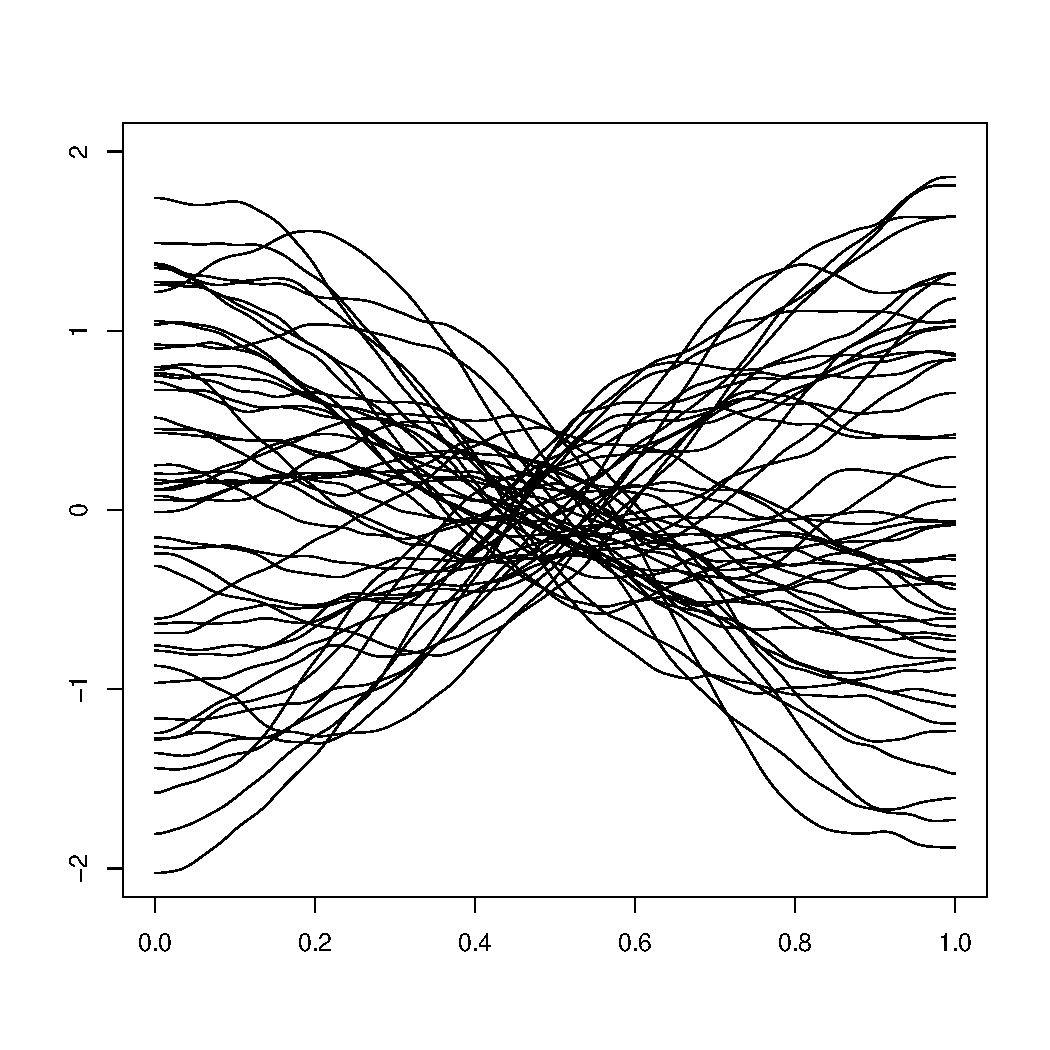
\includegraphics[width=\textwidth]{Images-nonparametric/cy-curves.pdf}
                \caption{}
        \end{subfigure}
         \begin{subfigure}[b]{0.24\textwidth}
                \centering
                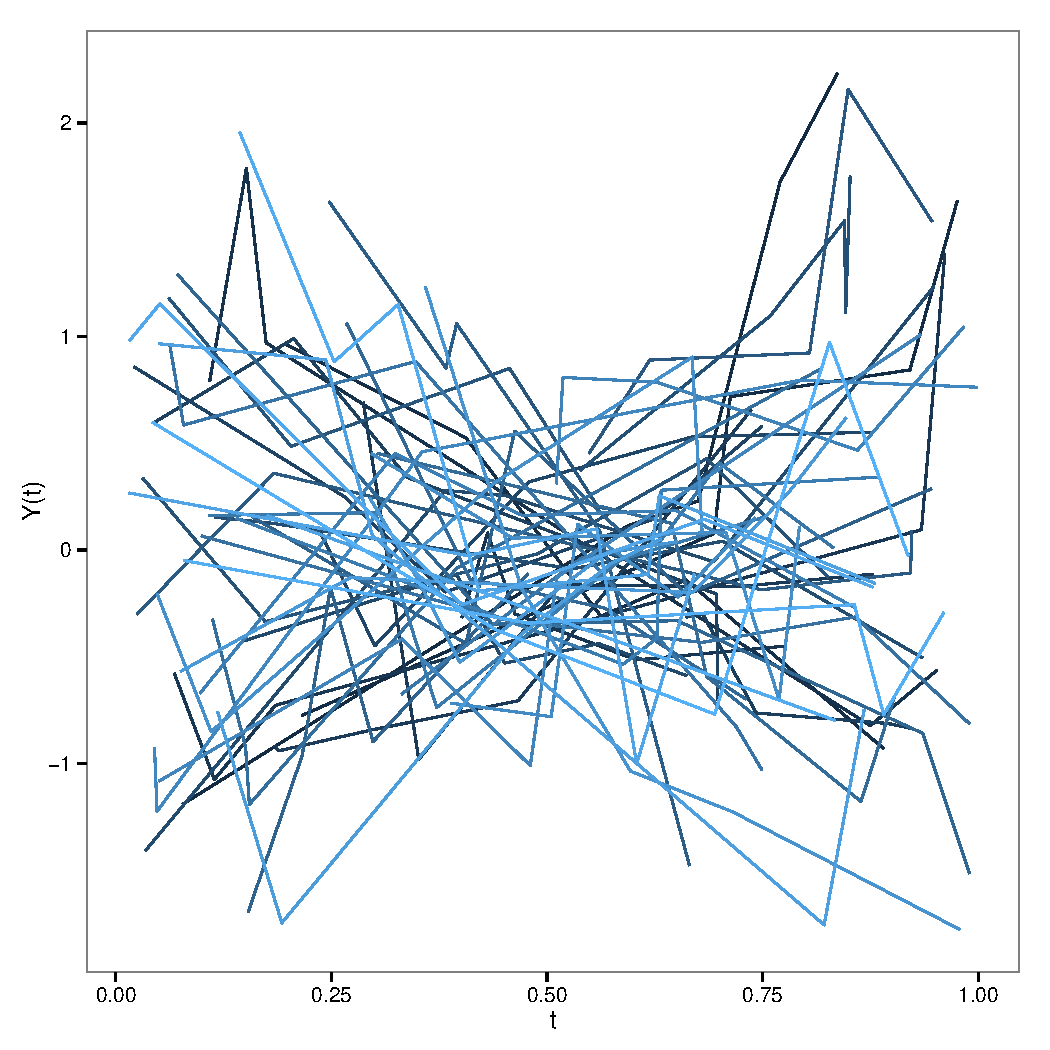
\includegraphics[width=\textwidth]{Images-nonparametric/cy-data-m5.pdf}
                \caption{}
                \label{}
        \end{subfigure}
        \begin{subfigure}[b]{0.24\textwidth}
                \centering
                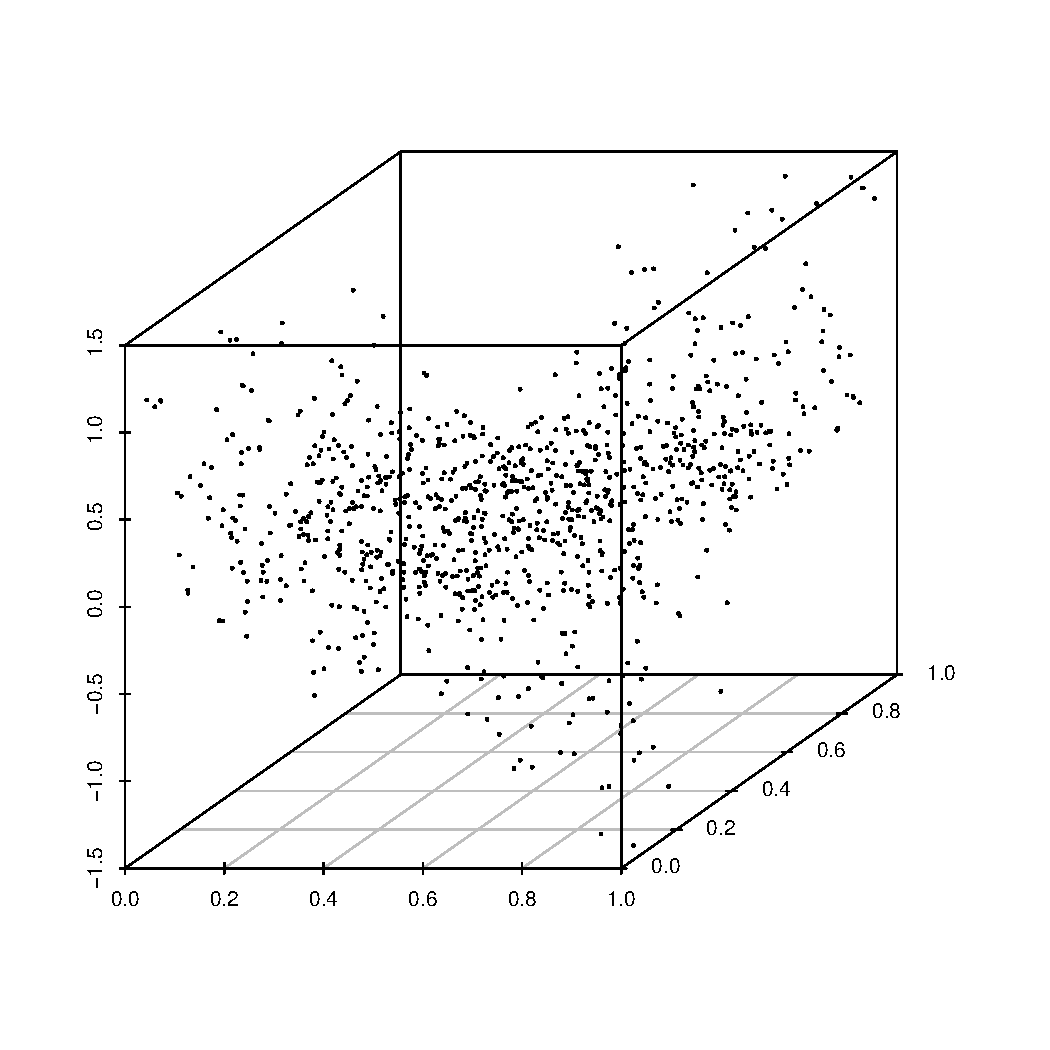
\includegraphics[width=\textwidth]{Images-nonparametric/cy-scatter3d-m5.pdf}
                \caption{}
                \label{}
        \end{subfigure}% 
          \begin{subfigure}[b]{0.24\textwidth}
                \centering
                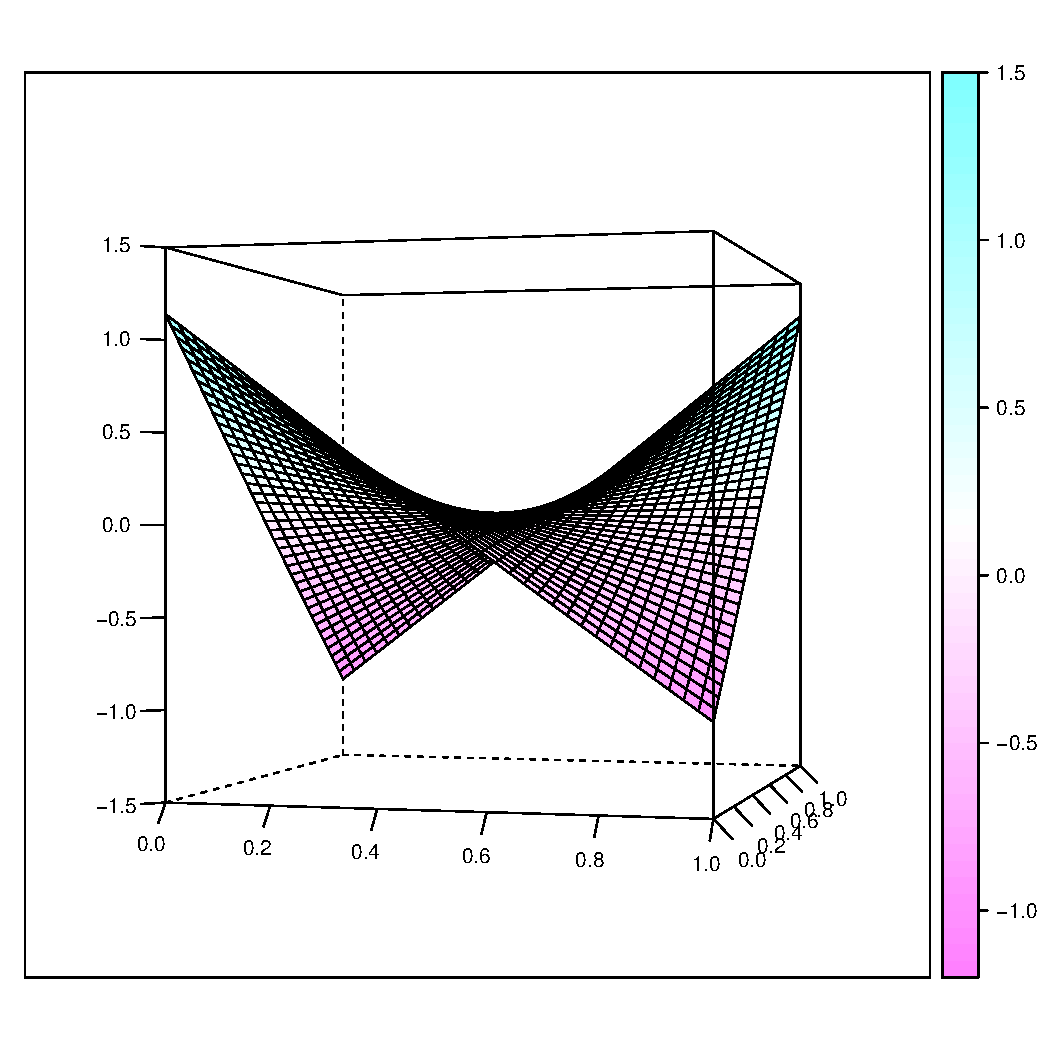
\includegraphics[width=\textwidth]{Images-nonparametric/cy-fit-wireframe-m5.pdf}
                \caption{}
                \label{}
        \end{subfigure}% 
        \caption{(a) 50 simulated curves from the process $X(t)$ in \eqref{eq:sim process} (b) data set of curves evaluated at five random locations with noise, $\sigma_0=0.392$ (c) Scatterplot of values based on the data used to estimate covariance surface (d) Estimated covariance function. }
        \label{fig:sim curves}
 \end{figure}
 
 \begin{figure}
 	\centering   
        \begin{subfigure}[b]{0.40\textwidth}
                \centering
                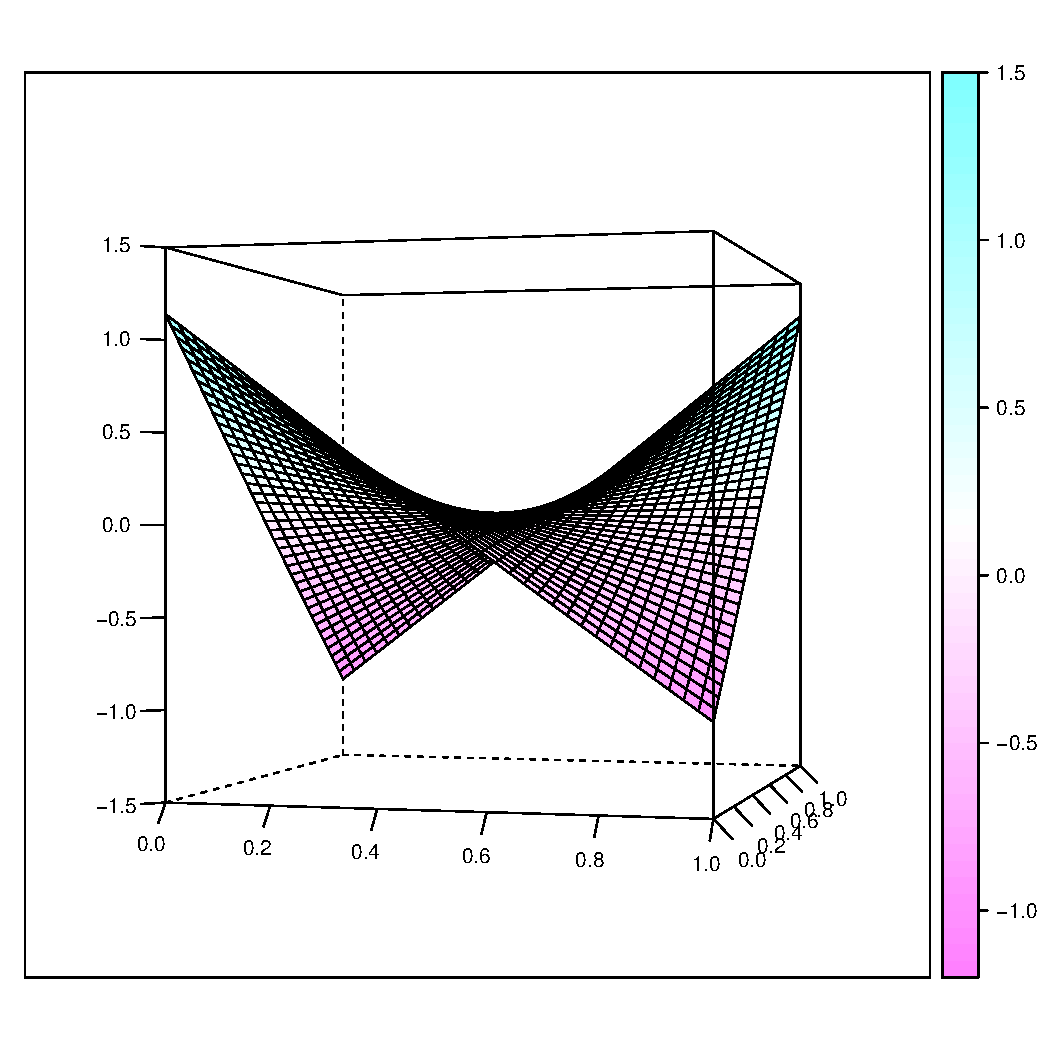
\includegraphics[width=\textwidth]{Images-nonparametric/cy-fit-wireframe-m5.pdf}
                \caption{m = 5}
                \label{}
        \end{subfigure}%
        \begin{subfigure}[b]{0.40\textwidth}
                \centering
                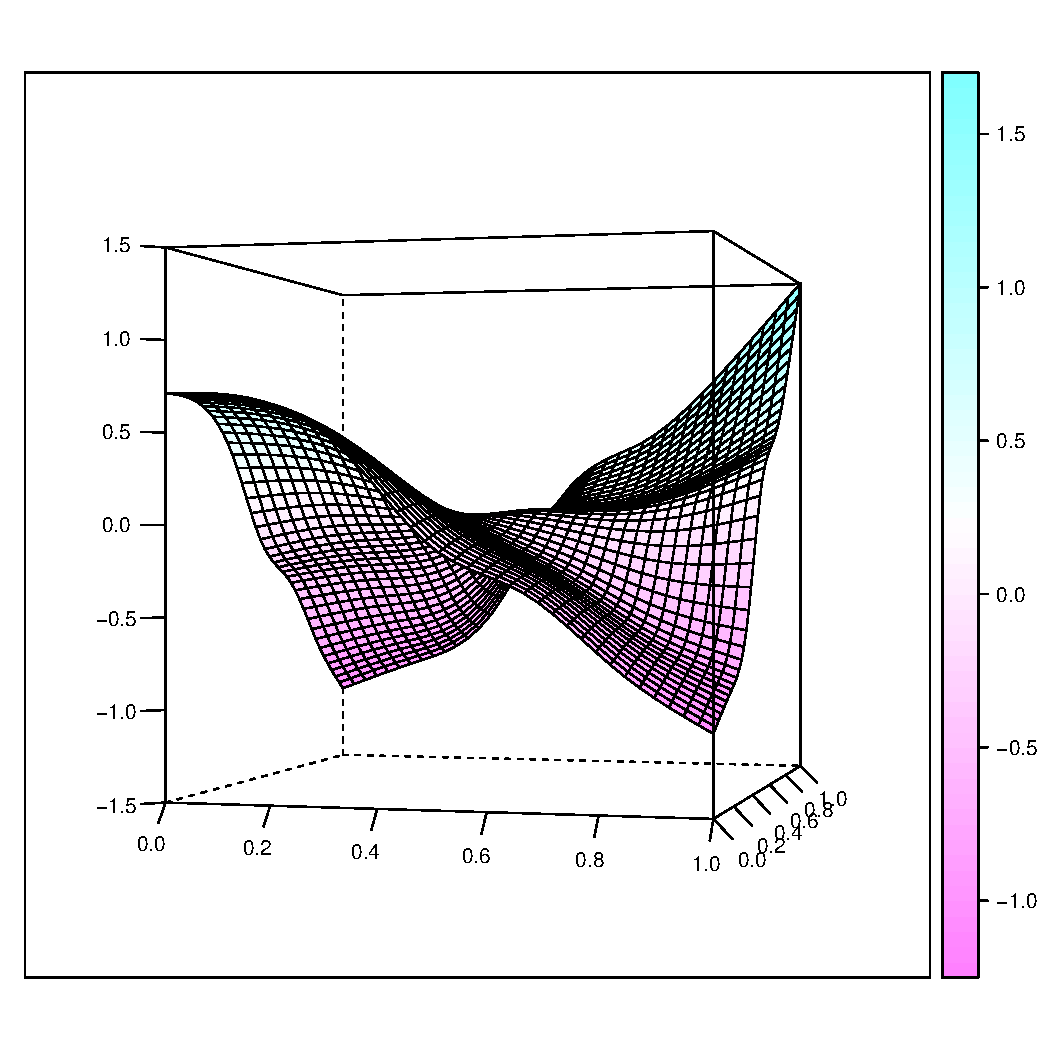
\includegraphics[width=\textwidth]{Images-nonparametric/cy-fit-wireframe-m10.pdf}
                \caption{m = 10}
                \label{}
        \end{subfigure}

        \begin{subfigure}[b]{0.40\textwidth}
                \centering
                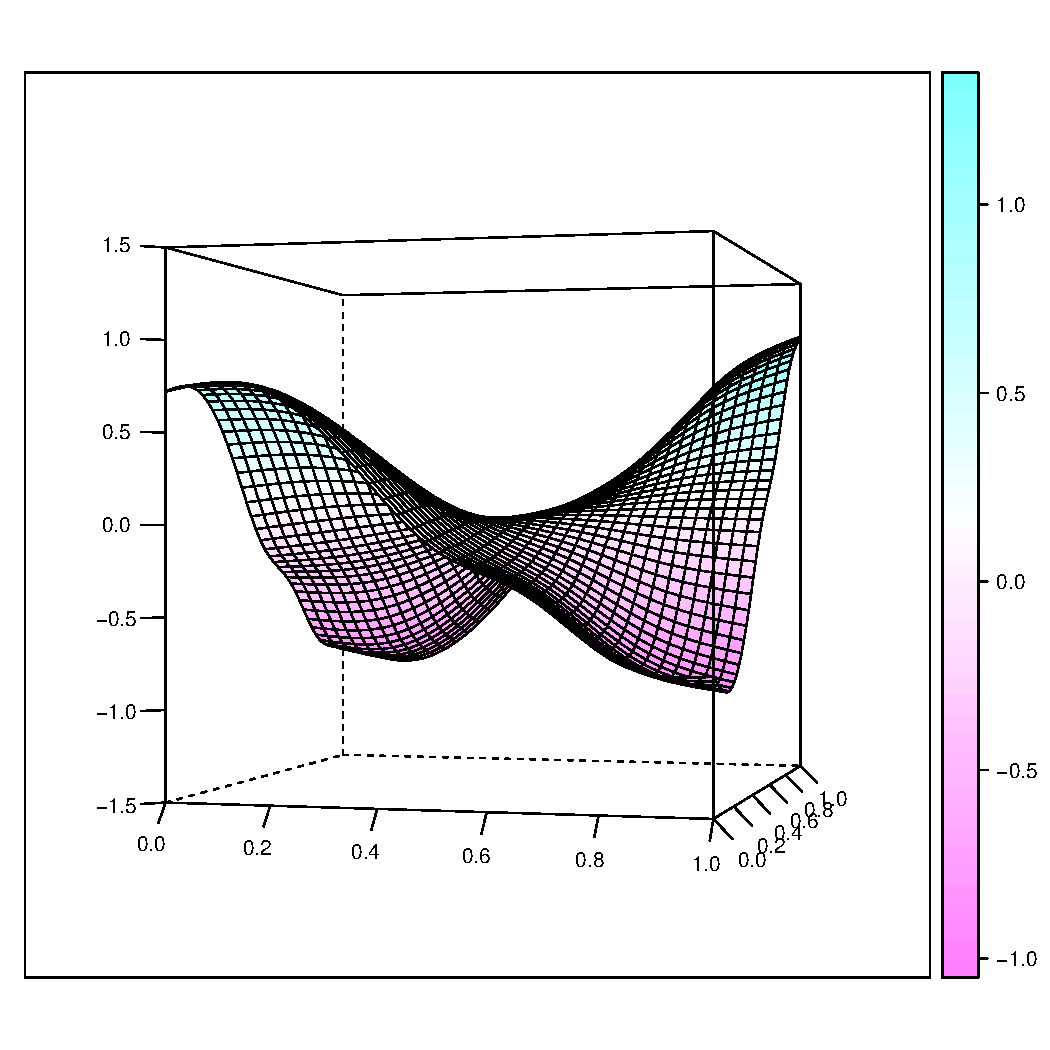
\includegraphics[width=\textwidth]{Images-nonparametric/cy-fit-wireframe-m40.pdf}
                \caption{m = 40}
                \label{}
        \end{subfigure}
                \begin{subfigure}[b]{0.40\textwidth}
                \centering
                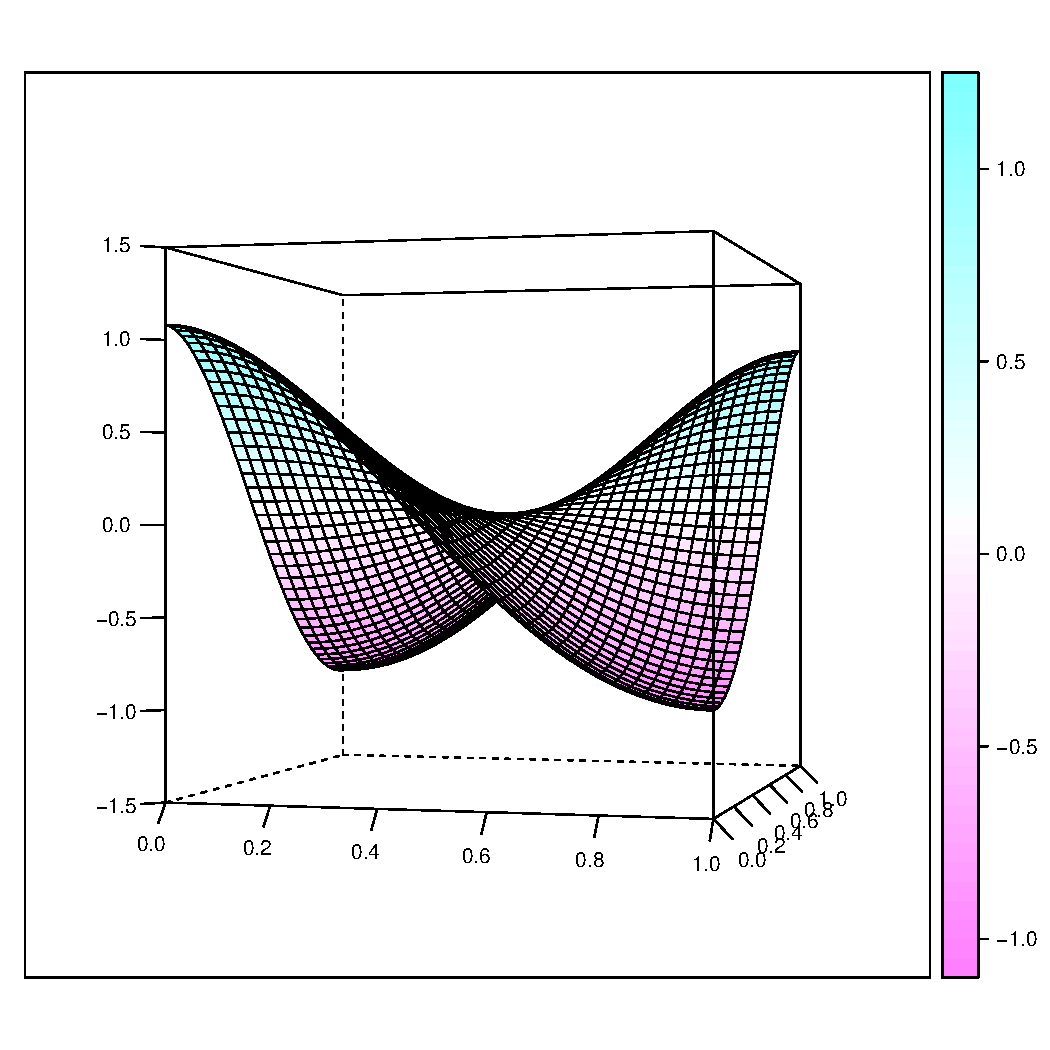
\includegraphics[width=\textwidth]{Images-nonparametric/cy-true-wireframe.pdf}
                \caption{truth}
                \label{}
        \end{subfigure}
        \caption{Estimated covariance functions based on the 50 curves simulated from the process $X(t)$ in \eqref{eq:sim process} using $\alpha=2$ and observation standard deviation equal to $\sigma_0 = 0.329$. (a) five observations per curve (b) ten observations per curve (c) forty observations per curve (d) true covariance functions }
        \label{fig:covfits}
\end{figure}

%\begin{figure}
%        \centering
%                \begin{subfigure}[b]{0.40\textwidth}
%                \centering
%                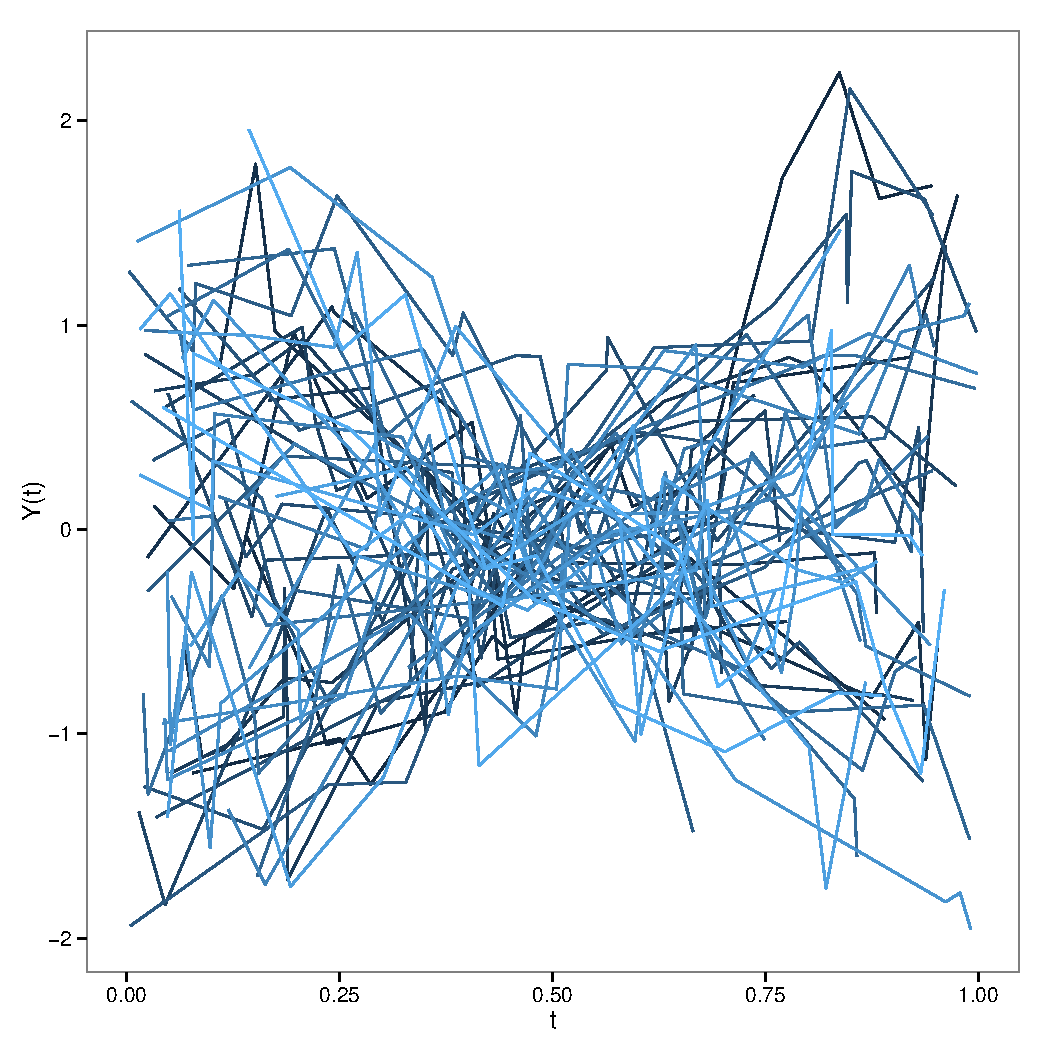
\includegraphics[width=\textwidth]{Images-nonparametric/cy-data-m10.pdf}
%                \caption{}
%                \label{}
%        \end{subfigure}
%        \begin{subfigure}[b]{0.40\textwidth}
%                \centering
%                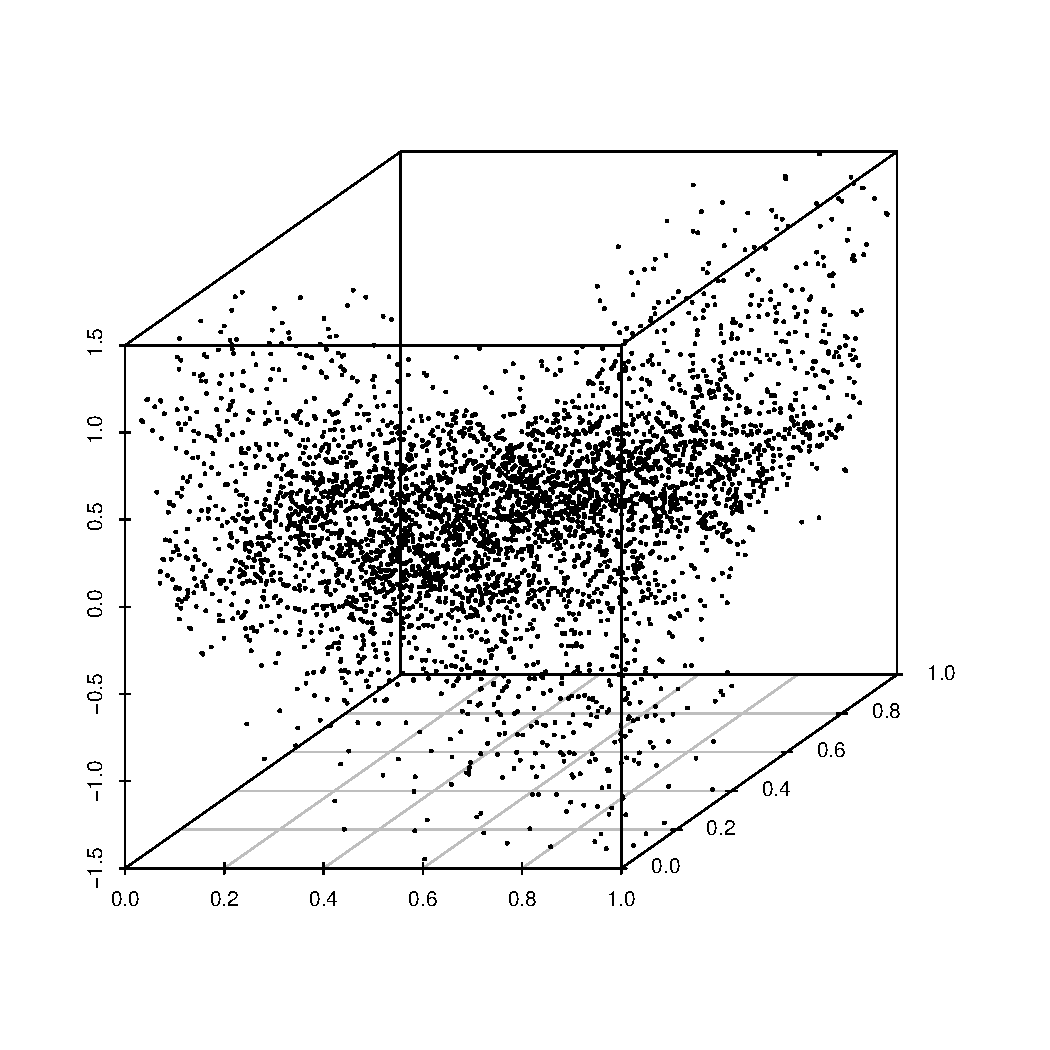
\includegraphics[width=\textwidth]{Images-nonparametric/cy-scatter3d-m10.pdf}
%                \caption{}
%                \label{}
%        \end{subfigure}% 
%        
%        \begin{subfigure}[b]{0.40\textwidth}
%                \centering
%                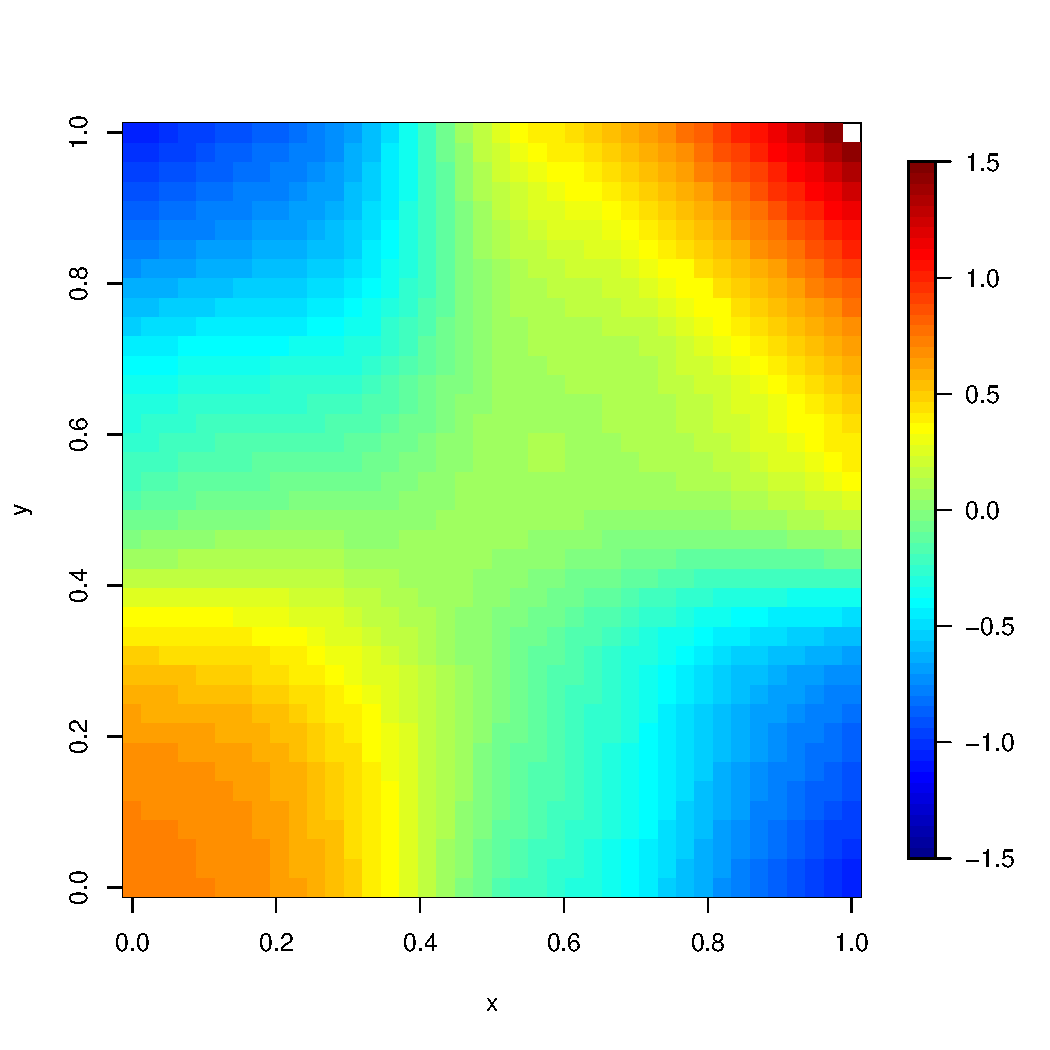
\includegraphics[width=\textwidth]{Images-nonparametric/cy-fit-image-m10.pdf}
%                \caption{m = 10}
%                \label{}
%        \end{subfigure}%
%        \begin{subfigure}[b]{0.40\textwidth}
%                \centering
%                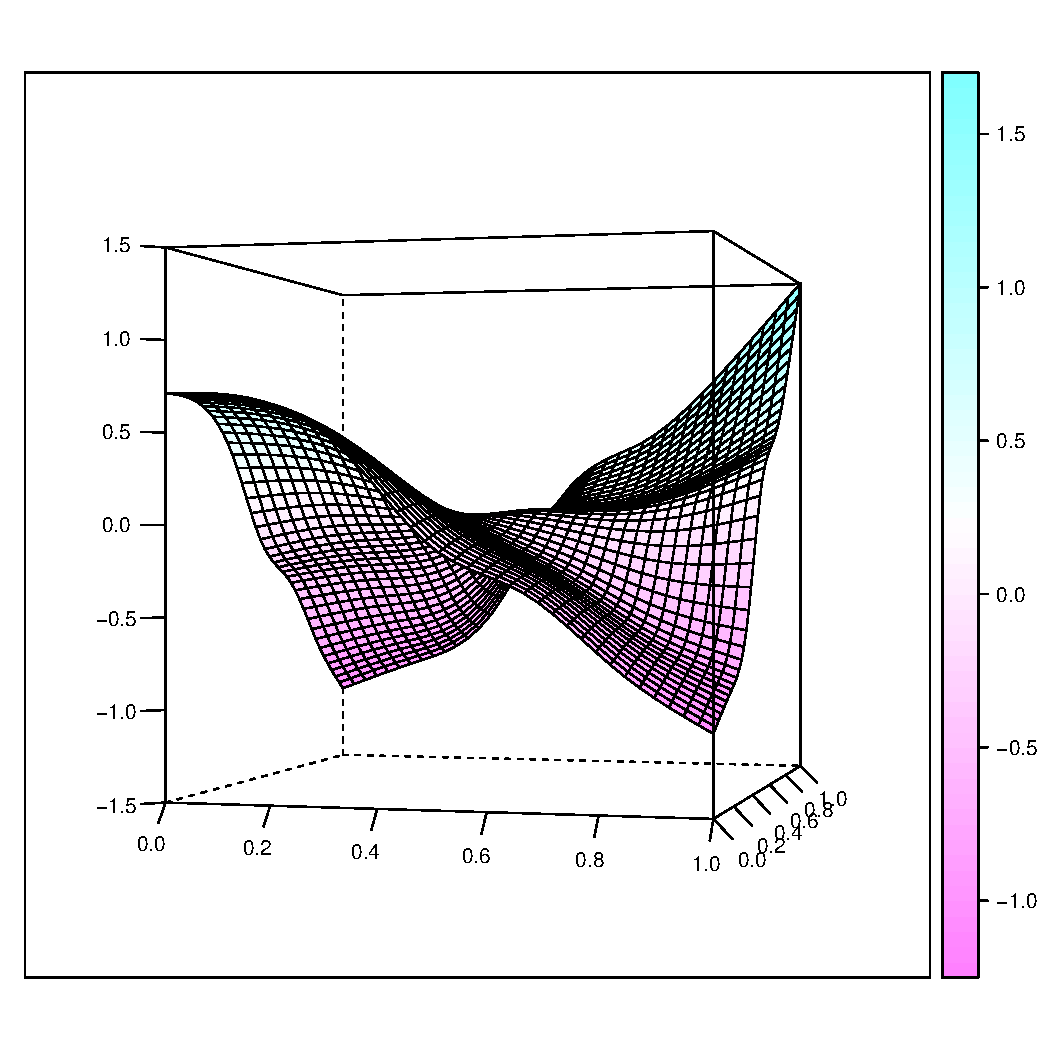
\includegraphics[width=\textwidth]{Images-nonparametric/cy-fit-wireframe-m10.pdf}
%                \caption{m = 10}
%                \label{}
%        \end{subfigure}
%
%        \begin{subfigure}[b]{0.40\textwidth}
%                \centering
%                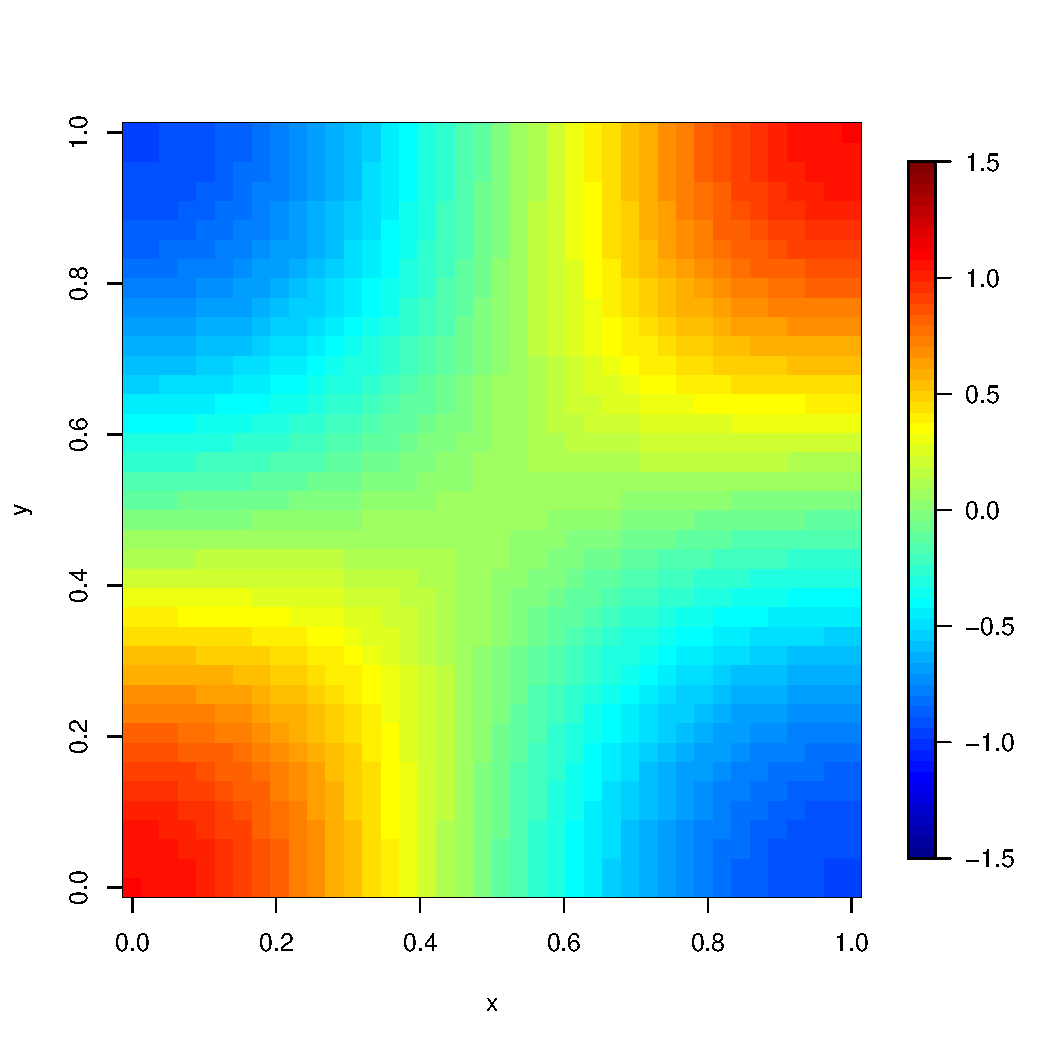
\includegraphics[width=\textwidth]{Images-nonparametric/cy-true-image.pdf}
%                \caption{truth}
%                \label{}
%        \end{subfigure}
%                \begin{subfigure}[b]{0.40\textwidth}
%                \centering
%                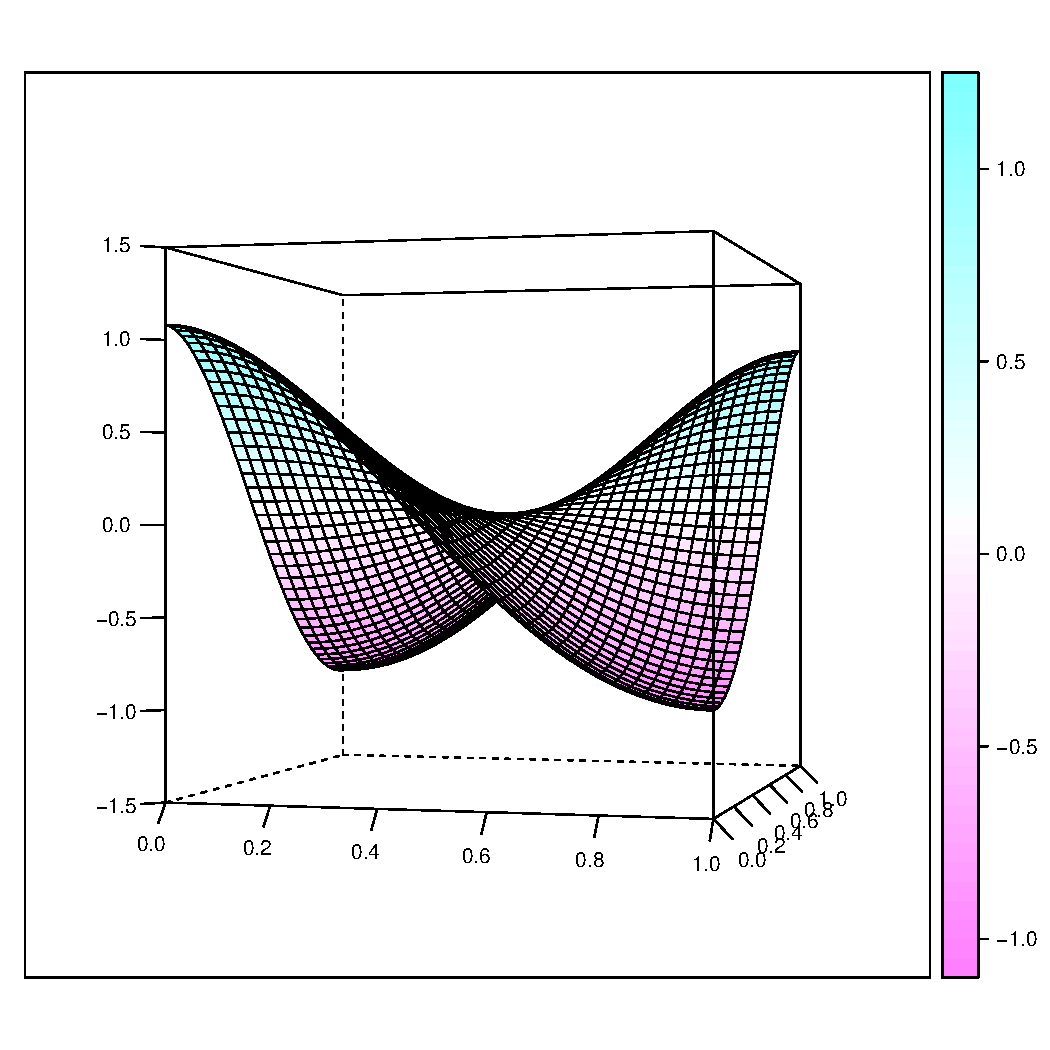
\includegraphics[width=\textwidth]{Images-nonparametric/cy-true-wireframe.pdf}
%                \caption{truth}
%                \label{}
%        \end{subfigure}
%        \caption{}\label{}
%\end{figure}

%\begin{figure}
%        \centering
%%                \begin{subfigure}[b]{0.40\textwidth}
%%                \centering
%%                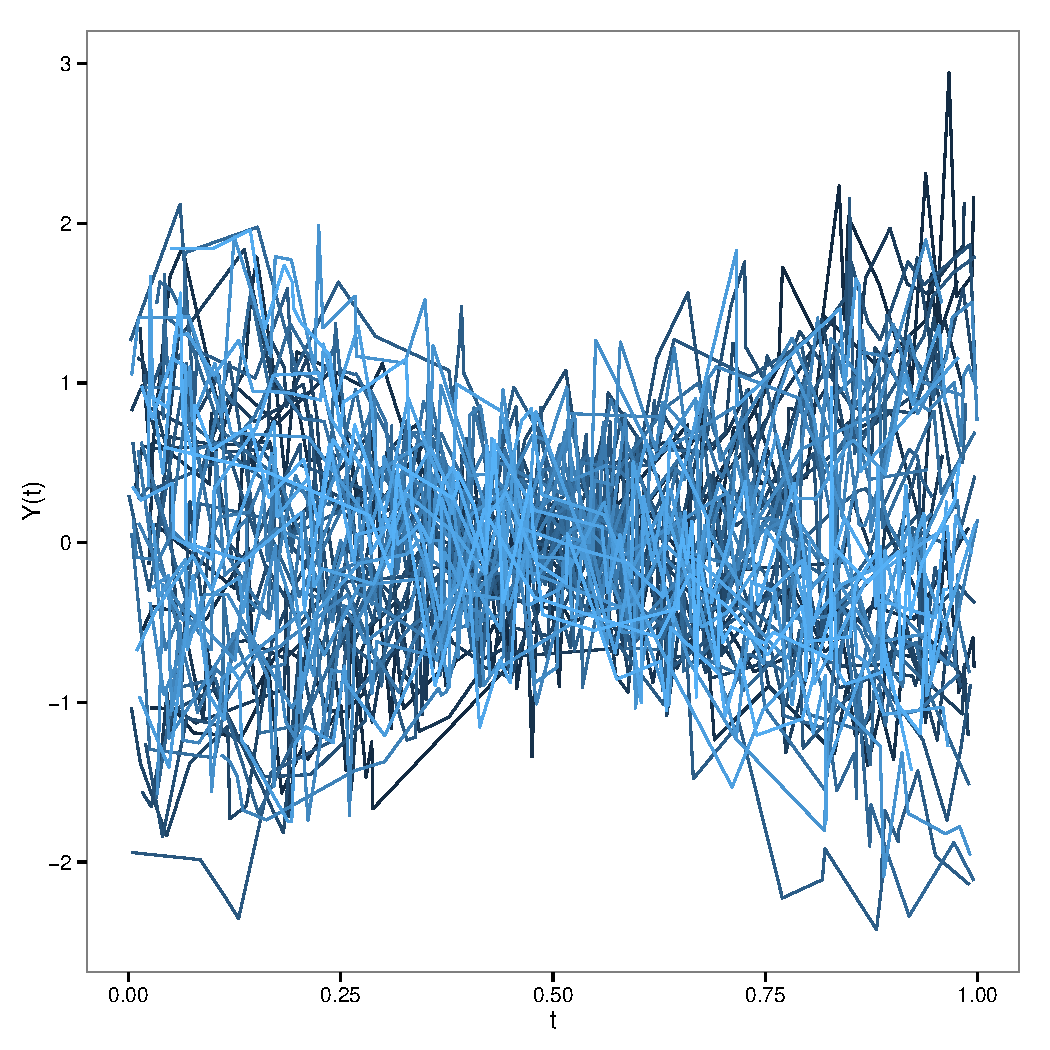
\includegraphics[width=\textwidth]{Images-nonparametric/cy-data-m40.pdf}
%%                \caption{}
%%                \label{}
%%        \end{subfigure}
%%        \begin{subfigure}[b]{0.40\textwidth}
%%                \centering
%%                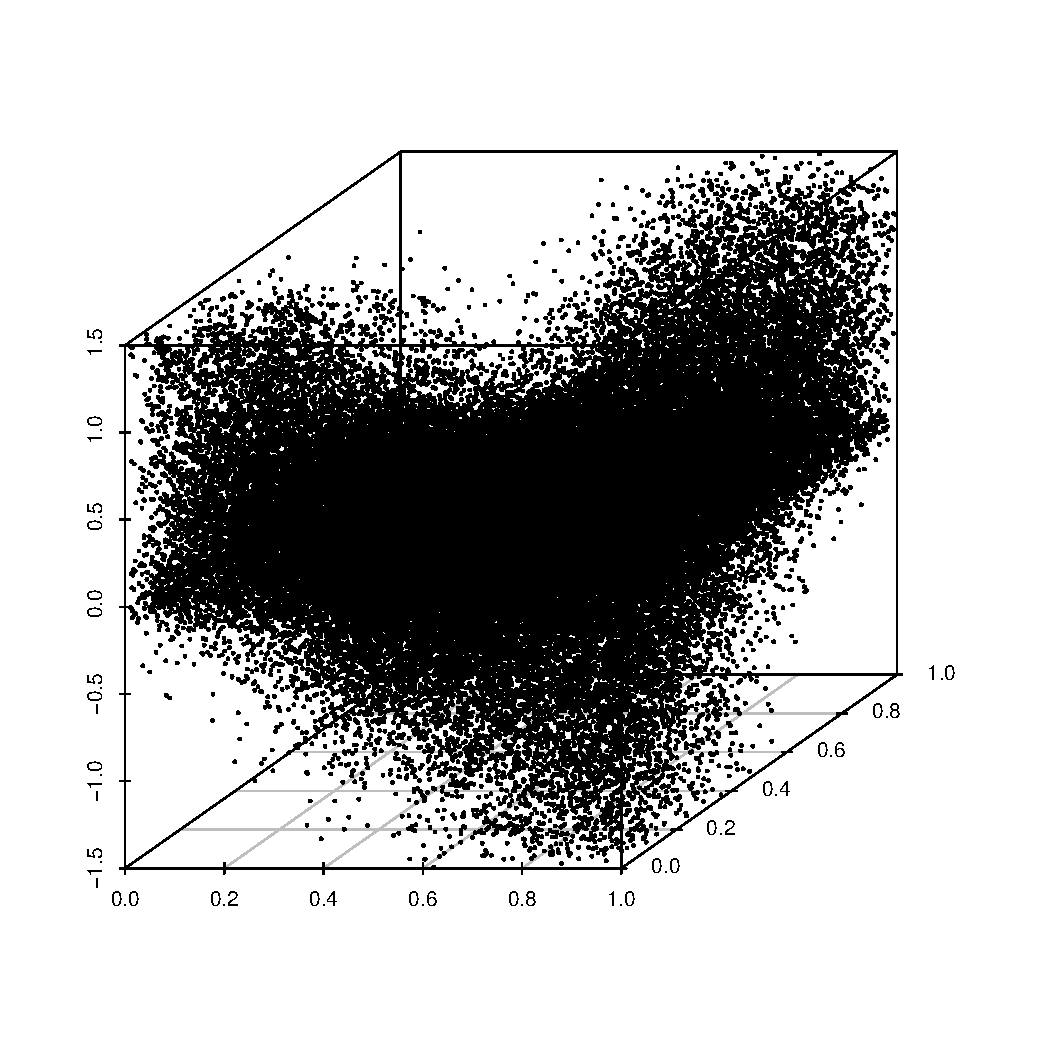
\includegraphics[width=\textwidth]{Images-nonparametric/cy-scatter3d-m40.pdf}
%%                \caption{}
%%                \label{}
%%        \end{subfigure}% 
%        
%        \begin{subfigure}[b]{0.40\textwidth}
%                \centering
%                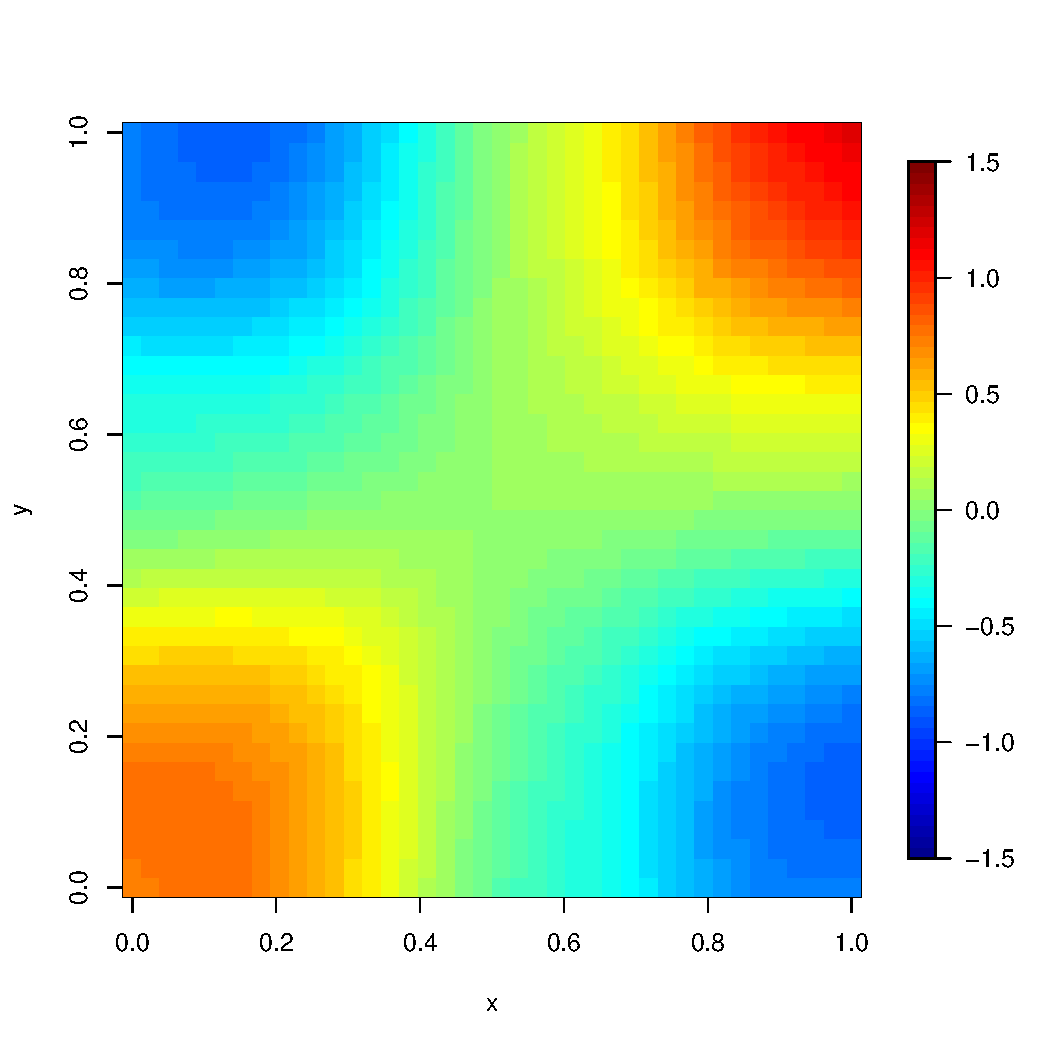
\includegraphics[width=\textwidth]{Images-nonparametric/cy-fit-image-m40.pdf}
%                \caption{m = 40}
%                \label{}
%        \end{subfigure}%
%        \begin{subfigure}[b]{0.40\textwidth}
%                \centering
%                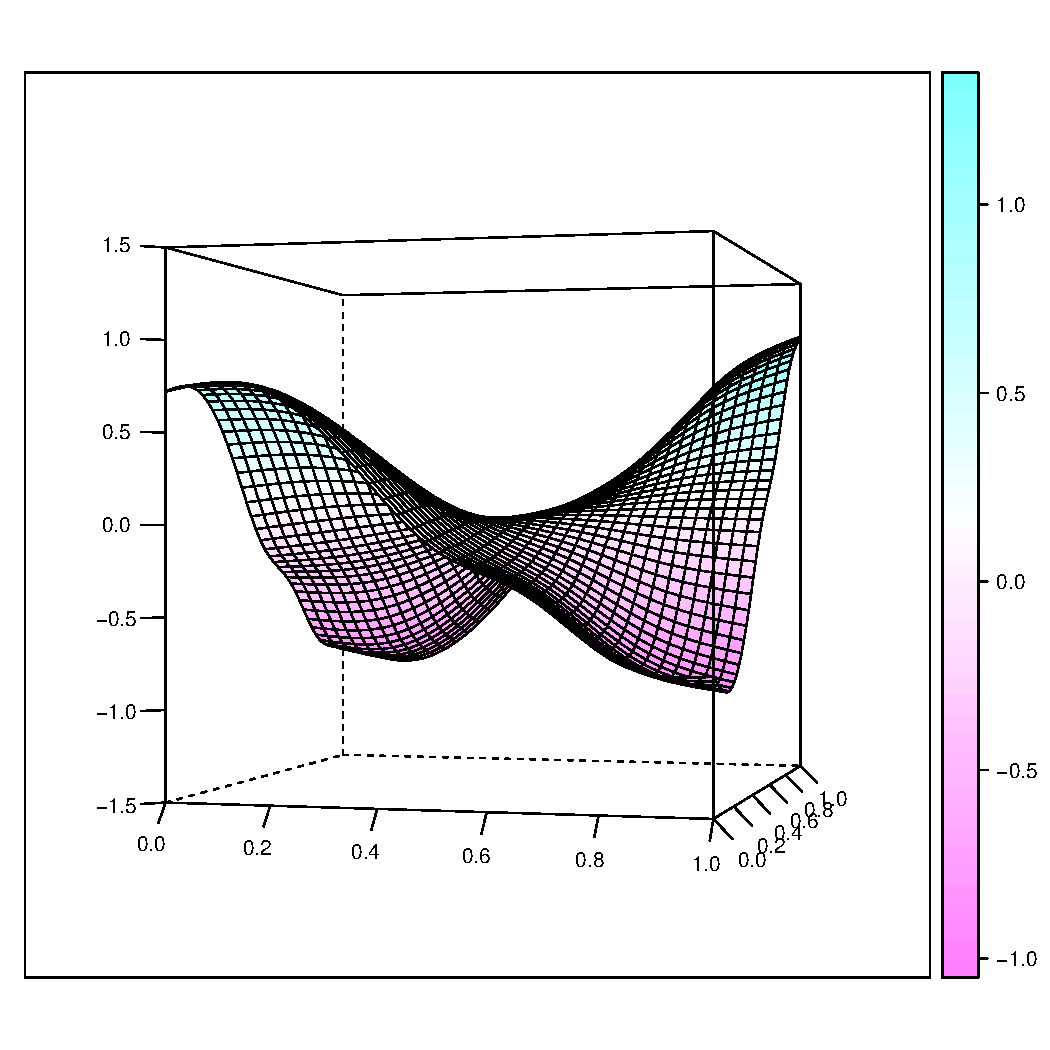
\includegraphics[width=\textwidth]{Images-nonparametric/cy-fit-wireframe-m40.pdf}
%                \caption{ m = 40}
%                \label{}
%        \end{subfigure}
%
%        \begin{subfigure}[b]{0.40\textwidth}
%                \centering
%                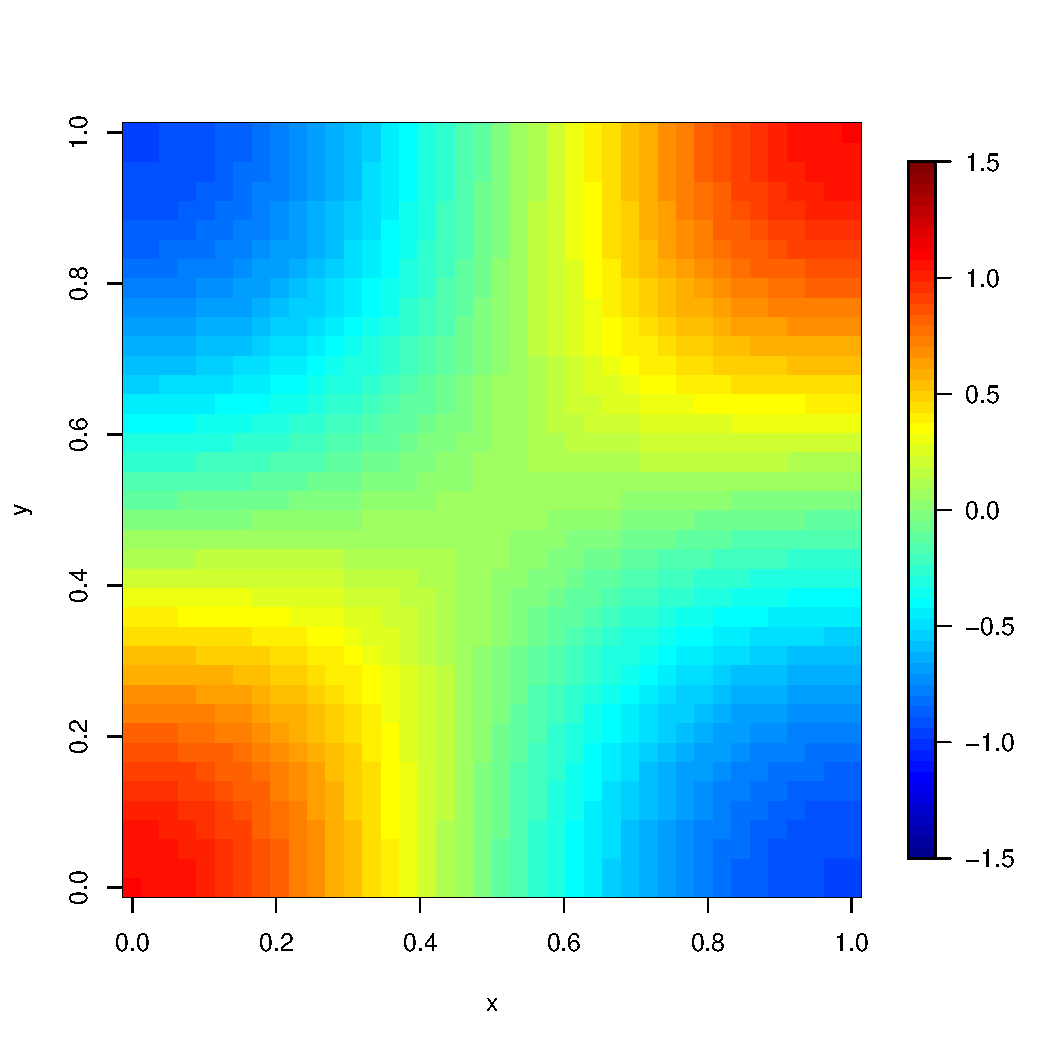
\includegraphics[width=\textwidth]{Images-nonparametric/cy-true-image.pdf}
%                \caption{truth}
%                \label{}
%        \end{subfigure}
%                \begin{subfigure}[b]{0.40\textwidth}
%                \centering
%                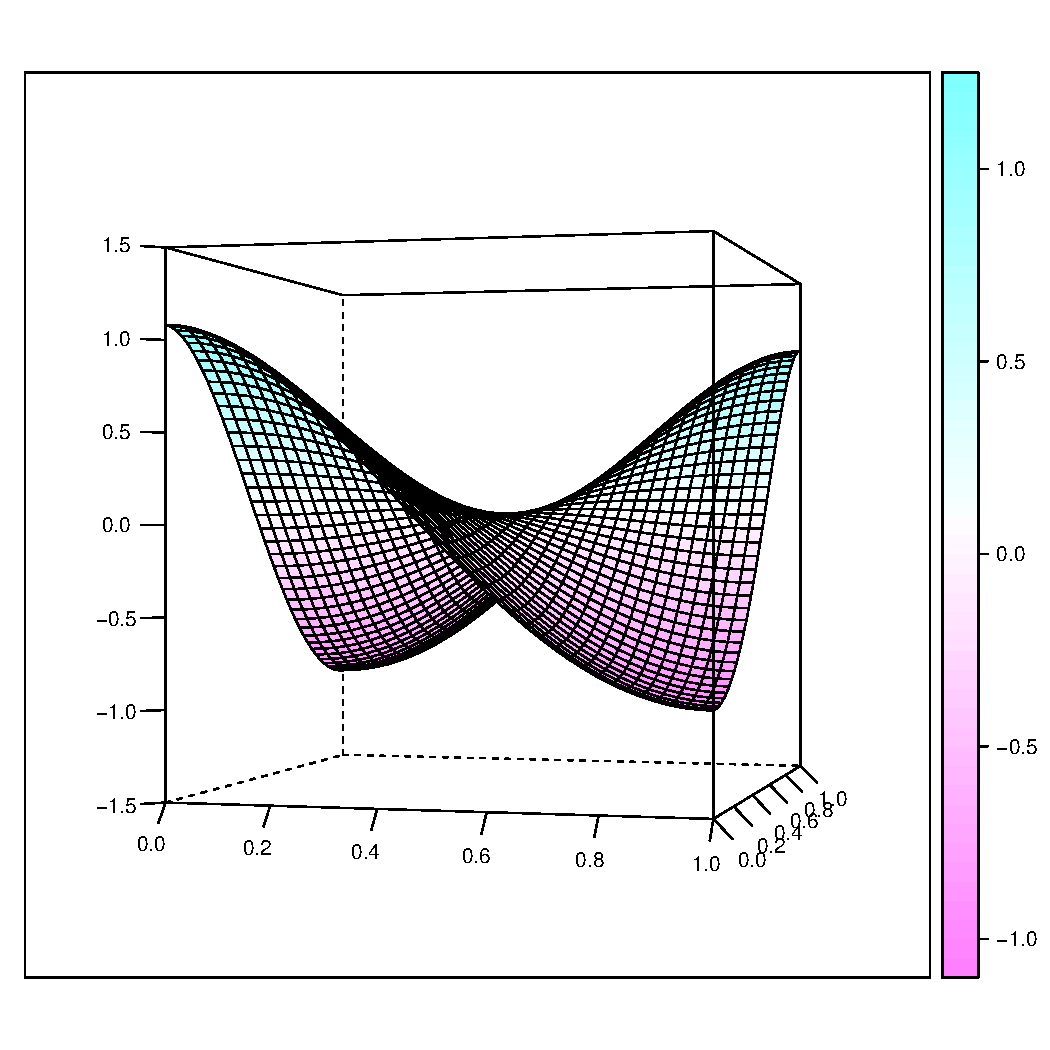
\includegraphics[width=\textwidth]{Images-nonparametric/cy-true-wireframe.pdf}
%                \caption{truth}
%                \label{}
%        \end{subfigure}
%        \caption{}\label{}
%\end{figure}




\section{Discussion} \label{covariance estimation: discussion}

We have shown how the reproducing kernel Hilbert space framework for covariance estimation can be extended to include unpenalized subspaces. We have also derived the form of the principal component functions. We believe that this is a more attractive framework because it allows smoothing penalties to be defined for larger function spaces. Simulation results indicate the estimator performs well even with sparsely observed curves. Even though development here was for a specific penalty, the method is very general and could easily be applied to other penalties, though the form of the reproducing kernel and the basis for the null space will depend on this choice. We have also created an R package implementation of this method with user-friendly functions for estimating the covariance function and principal component functions for functional data, making it convenient to use empirical basis representation for functional data analyses. Documentation for the R package is included in appendix. 



%\begin{figure}[htbp]
%\begin{center}
%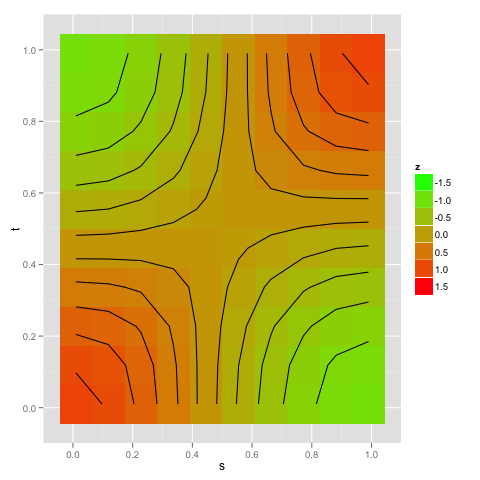
\includegraphics[width = 0.5\textwidth ]{images/Ch3/covfun.png}
%\caption{Covariance function}
%\label{default}
%\end{center}
%\end{figure}



%\begin{figure}[htbp]
%\begin{center}
%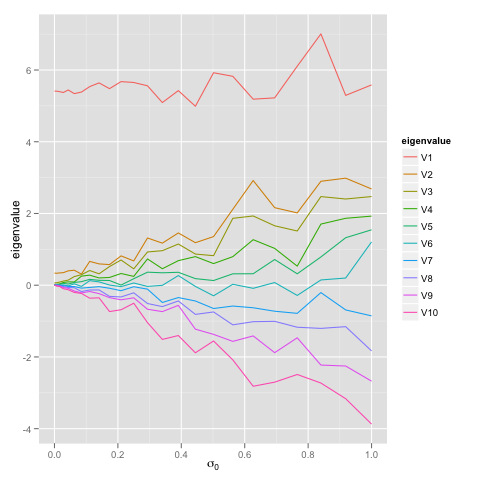
\includegraphics[width = 0.8\textwidth ]{images/Ch3/eval-seq.png}
%\caption{default}
%\label{default}
%\end{center}
%\end{figure}
%
%\begin{figure}[htbp]
%\begin{center}
%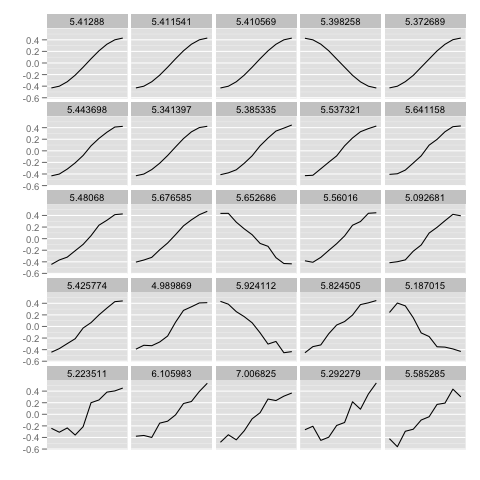
\includegraphics[width = 0.8\textwidth ]{images/Ch3/first-efun.png}
%\caption{default}
%\label{default}
%\end{center}
%\end{figure}
%
%\begin{figure}[htbp]
%\begin{center}
%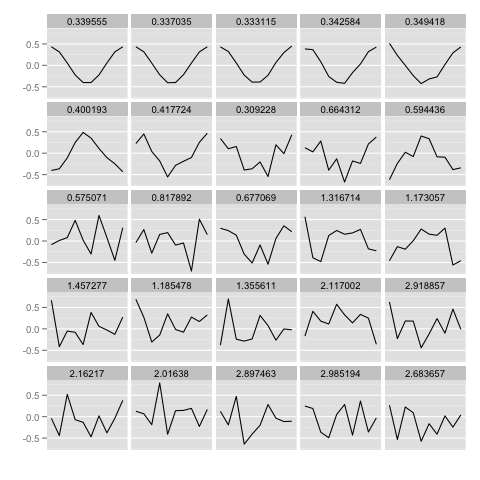
\includegraphics[width = 0.8\textwidth ]{images/Ch3/second-efun.png}
%\caption{default}
%\label{default}
%\end{center}
%\end{figure}




